Este capítulo tem como objetivo consolidar a linha de raciocínio fundamental para a elaboração desta dissertação. Primeiramente, apresenta-se um panorama geral sobre o agronegócio brasileiro, com foco na cultura do algodão, abordando pontos como os principais desafios da produção, sua importância e seus destinos comerciais. Em seguida, o texto detalha o processo de avaliação da qualidade do algodão, com ênfase nos padrões internacionais, regulamentações específicas no Brasil e os processos adotados na indústria. Na sequência, contextualiza-se o tema dos sistemas de visão computacional, com aplicações no setor da agricultura, especialmente na classificação automatizada. Por fim, o capítulo discute o papel da inteligência artificial e  os principais modelos empregados em sistemas de visão computacional, culminando na identificação da lacuna de pesquisa que este trabalho se propõe a preencher.

\section{Agronegócio Brasileiro e o Algodão}
\label{sec:agro_brasileiro_algodao}

Esta seção apresenta a fundamentação teórica sobre a cadeia produtiva do algodão no Brasil, contextualizando o cenário onde a solução proposta nesta dissertação foi aplicada. Para o desenvolvimento de sistemas de visão computacional eficazes na classificação de fibras naturais, é imprescindível compreender a origem dos defeitos visuais e das impurezas que determinam a classificação da qualidade. Dessa forma, as subseções a seguir mapeiam o fluxo agroindustrial, desde a colheita mecanizada e o beneficiamento até os gargalos logísticos, identificando como cada etapa do processo produtivo influencia as propriedades físicas da pluma e impõe desafios específicos à classificação automática da qualidade da fibra do algodão.

% Revisado

\subsection{Agricultura no Brasil}
\label{subsec:agricultura_brasil}

    A agricultura brasileira já se consolidou como uma das maiores do mundo, fornecendo produtos essenciais para diversos setores da economia global, como a alimentação, a bioenergia, o setor têxtil, entre outros. Essa consolidação é um reflexo de investimentos em inovações tecnológicas, que começaram com a terceira revolução agrícola (Revolução Verde) e se estendem até hoje com a disseminação da agricultura digital, integrando a agricultura de precisão e ferramentas como inteligência artificial para aumento da produtividade e sustentabilidade \cite{abbade2014agro, basso2024agriculture}.

    O setor tem se destacado como um dos mais robustos, representando 23\% da economia nacional \cite{filho2024pib}, com exportações atingindo recordes históricos. Mesmo em cenários de queda nos preços das commodities e desafios climáticos(como secas e o fenômeno El Niño \cite{lin2019elnino}) e gargalos logísticos \cite{goncalves2024logistica}, o Brasil manteve o crescimento no valor total exportado. Em 2024, a expectativa é de que o país alcance US\$ 168,1 bilhões em exportações de produtos agrícolas, impulsionado por fatores como a desvalorização do real frente ao dólar, o que aumenta a competitividade dos produtos brasileiros no mercado internacional \cite{cardoso2024perspectivas}.

    No contexto da produção agrícola brasileira, a tecnologia desempenhou um papel essencial na adaptação do país a diferentes tipos de culturas, permitindo o cultivo de variedades mais resistentes e otimizadas para o clima tropical \cite{basso2024agriculture}. Além disso, a introdução de biotecnologia e o avanço em estudos moleculares têm possibilitado o desenvolvimento de culturas com maior produtividade e resistência a pragas \cite{das2023biotech}, sendo o algodão (\textit{Gossypium hirsutum}) um exemplo significativo, cuja produção se beneficia de tais avanços, como resistência genética e técnicas de cultivo adaptadas ao clima e solo brasileiros \cite{ribeiro2017cottontrans, ribeiro2019cottontrans, ribeiro2023cottontrans}.

\subsection{A Cadeia Produtiva do Algodão}
\label{subsec:cadeia_algodao}

    Em 2024, o Brasil se consolidou como o maior exportador mundial de algodão em volume. As condições climáticas favoráveis, aliadas ao aumento da demanda internacional, permitiram um crescimento expressivo das exportações brasileiras de algodão. A produção alcançou 3,2 milhões de toneladas, com a China como principal destino, e as exportações estão projetadas para somar US\$ 5,2 bilhões até o fim do ano, um aumento de 56\% em relação ao ano anterior. Isso reflete o papel estratégico do algodão na pauta exportadora do agronegócio brasileiro, que vai além da alimentação, abrangendo setores como o têxtil e de bioenergia \cite{cardoso2024perspectivas}.

    A cadeia produtiva do algodão é caracterizada por um fluxo agroindustrial complexo, no qual a valoração final do produto depende intrinsecamente da preservação das características da fibra ao longo das etapas de produção, beneficiamento e classificação. A seguir, descrevem-se as etapas críticas que influenciam a qualidade visual e intrínseca da pluma.

    \subsubsection{Produção no Campo: O Impacto da Colheita na Pureza da Fibra}

        A qualidade da fibra de algodão começa no manejo da lavoura. Fatores de estresse abiótico e o manejo da desfolha influenciam diretamente parâmetros fisiológicos da planta, determinando a maturidade e a resistência da fibra colhida \cite{sezener2021cotton}.

        No entanto, um dilema crítico para a classificação visual reside na natureza do método de colheita. Em Mato Grosso, estado responsável por mais de 56\% da produção nacional, a colheita é plenamente mecanizada. Embora o sistema de fusos (\textit{picker}) seja majoritário devido à sua seletividade superior, o sistema de arranque (\textit{stripper}) ainda é utilizado em nichos de cultivo adensado visando a redução de custos operacionais. Independentemente do maquinário, a mecanização impõe um \textit{trade-off} na qualidade: \citeonline{ferreira2013sistemas} destacam que, enquanto a colheita manual apresenta perdas e impurezas em torno de 5\%, a colheita mecânica eleva esse patamar para 15 a 17\%.

        Essa carga de material estranho impacta diretamente a análise automática. A ação mecânica, mesmo no sistema \textit{picker}, introduz contaminantes biológicos e promove a formação de \textit{neps}, fenômeno exacerbado no sistema \textit{stripper}, que agrega cascas, galhos, folhas e brácteas à pluma \cite{kazama2016influencia, silva2007colheita}. A presença destes contaminantes heterogêneos é descrita por \citeonline{ferreira2013sistemas} como a responsável pela redução da reflectância e aumento do amarelamento da pluma, o que define a complexidade do problema para sistemas de visão computacional. Diferente de ambientes controlados, a classificação automática exige algoritmos robustos capazes de realizar a segmentação semântica da fibra valiosa em meio a esse ``ruído'' vegetal e às oclusões geradas pelo processo de extração mecânica.

    \subsubsection{Beneficiamento (Algodoeira): O Processo de Limpeza}

        Após a colheita, o algodão em caroço é transportado para a Unidade de Beneficiamento. Essa etapa configura-se como o elo de ligação entre a produção agrícola e a indústria têxtil, sendo fundamental para a preservação das qualidades intrínsecas da fibra. Segundo \citeonline{ferreira2022cadeia}, o beneficiamento moderno no Brasil passou por profundas transformações tecnológicas, substituindo modelos obsoletos por parques fabris empresariais focados em atender à demanda internacional por qualidade e rastreabilidade.

        O fluxo operacional nessas unidades visa separar a fibra da semente e remover as impurezas trazidas do campo. Conforme detalhado tecnicamente por \citeonline{silva2010impacto} ao analisarem algodoeiras em Mato Grosso, o processo típico envolve:

        \begin{itemize}
            \item \textbf{Pré-limpeza:} Sistemas de extração e batedores que removem impurezas grosseiras (cascas e galhos) antes que o algodão entre nos descaroçadores.
            
            \item \textbf{Descaroçamento:} O ponto crítico do processo, no qual serras mecânicas separam a fibra do caroço. É nesta etapa que ocorre o maior estresse na fibra, podendo elevar a formação de \textit{neps} em até 80\%.

            \item \textbf{Limpeza de Pluma:} Uso de equipamentos como o \textit{Constelation} e fluxos de ar para expulsar a sujeira fina (poeira). Embora aumente a limpeza visual, o excesso de processamento mecânico aqui pode romper fibras e agravar a contagem de \textit{neps}.
        \end{itemize}

        Apesar da modernização citada por \citeonline{ferreira2022cadeia}, a remoção mecânica de impurezas não ocorre sem prejuízos à integridade da pluma: o processo é eficaz na limpeza, mas acaba fragmentando contaminantes maiores em partículas minúsculas (\textit{pepper trash}), dificultando sua detecção posterior por métodos tradicionais \cite{mustafic2016}. Para sistemas de visão computacional, isso resulta em um panorama desafiador, em que a distinção entre uma impureza vegetal fragmentada e um emaranhado de fibra exige alta precisão de detecção.


    \subsubsection{Classificação Comercial e Rastreabilidade}

        Após o beneficiamento e a prensagem, o algodão passa pela etapa de classificação, que vai além da simples verificação técnica para atuar como o mecanismo central de regulação comercial. Conforme destacado por \citeonline{martins2020qualidade}, a qualidade da fibra é o fator determinante para a precificação, definindo se o lote receberá ágio ou deságio sobre o preço-base de mercado (como o índice CEPEA/ESALQ), dependendo de seus atributos intrínsecos (comprimento, resistência, micronaire) e extrínsecos (impurezas e cor).

        Para mitigar a subjetividade da análise visual humana, o setor consolidou o uso de instrumentos de HVI (\textit{High Volume Instrument}). Segundo o relatório da \citeonline{itmf2025brazil}, a padronização via HVI foi crucial para que o Brasil deixasse de ser visto apenas como um fornecedor de \textit{commodity} e passasse a competir em mercados \textit{premium}. No entanto, o custo operacional dessa instrumentação e o tempo de análise a tornam inviável para o controle logístico de emblocamento em tempo real. Além disso, a variabilidade no campo ainda impõe barreiras severas: \citeonline{souza2021perdas} demonstram que fatores como o tempo de exposição da fibra às intempéries e o atraso na colheita degradam significativamente os parâmetros de Cor (\textit{Color Grade}) e aumentam o índice de Impurezas (\textit{Trash}), comprometendo a classificação final e gerando prejuízos industriais.

        Paralelamente à classificação, a rastreabilidade tornou-se um requisito não tarifário para a exportação. O Sistema Abrapa de Identificação (SAI) evoluiu para integrar dados de campo e indústria. De acordo com análise técnica de \citeonline{lima2025blockchain}, o uso de tecnologias como \textit{blockchain} no SAI garante a imutabilidade dos dados, permitindo que cada fardo carregue uma ``identidade digital'' auditável desde a fazenda até a fiação.

        Recentemente, essa rastreabilidade foi ampliada pelo programa ``SouABR'', que conecta a ponta produtiva ao varejo de moda. Segundo estudo da \citeonline{fgv2022rastreabilidade}, essa iniciativa permite que o consumidor final, via \textit{QR Code}, acesse o histórico completo da peça, certificando a origem sustentável e as características técnicas da fibra utilizada.

        Uma análise aprofundada sobre os parâmetros técnicos do HVI e os obstáculos computacionais da classificação visual será apresentada na Seção \ref{sec:qualidade}.

    \subsubsection{Armazenamento e Logística}

        A logística do algodão configura-se como o gargalo final da cadeia produtiva, especialmente no contexto atual no qual o Brasil consolidou-se como o maior exportador mundial da fibra. Segundo o levantamento oficial da \citeonline{conab2025boletim}, a superação dos Estados Unidos no ranking global de exportações impõe uma pressão inédita sobre a infraestrutura nacional, exigindo eficiência para escoar um volume recorde destinado majoritariamente aos mercados asiáticos.

        A primeira dificuldade crítica reside na etapa de armazenagem na origem. Diferente de outras commodities, o fardo de algodão exige condições específicas de temperatura e umidade para evitar a degradação da fibra. No entanto, \citeonline{lourenco2020capacidade} alertam para um déficit estrutural na capacidade estática de armazenagem em Mato Grosso. O estudo aponta que o crescimento da produção agrícola no estado foi muito superior ao investimento em armazéns, forçando o uso de pátios improvisados que expõem a pluma a riscos climáticos e dificultam a segregação dos lotes por qualidade visual e HVI.

        No transporte, a matriz brasileira permanece fortemente dependente do modal rodoviário para percorrer distâncias que frequentemente superam 2.000 km entre o Cerrado e os portos. Em uma análise recente sobre a infraestrutura do agronegócio, \citeonline{pera2025logistica} alerta que, na contramão das melhores práticas globais, o Brasil aumentou sua dependência de caminhões para o escoamento de safra (de 45\% para 54\% na última década), enquanto o uso de ferrovias recuou. Essa distorção estrutural, segundo o autor, torna o frete brasileiro significativamente mais oneroso e intensivo em carbono quando comparado aos competidores estadunidenses, que possuem uma matriz de transporte integrada e eficiente para o escoamento de suas commodities.

        Para mitigar a saturação histórica do Porto de Santos, novas rotas de escoamento ganharam relevância estratégica. O estudo técnico de \citeonline{coelho2025algodao}, publicado pelo Banco do Nordeste, destaca a ascensão do Porto de Salvador e dos terminais do Arco Norte como alternativas viáveis. Segundo o autor, a consolidação dessas rotas reduziu o tempo de trânsito para a Ásia e permitiu que a produção da Bahia e do norte de Mato Grosso escoasse com menor custo operacional.

        Essa descentralização é corroborada pelos dados da \citeonline{antaq2025anuario}, que registram um crescimento sustentado na movimentação de cargas conteinerizadas nos portos do Norte/Nordeste. A agência reguladora aponta que a diversificação portuária não é apenas uma questão econômica, mas uma necessidade de segurança logística para garantir o cumprimento dos contratos internacionais em prazos rígidos.

        Por fim, este cenário logístico complexo impõe um entrave adicional à garantia da qualidade. A longa exposição ao transporte rodoviário e o armazenamento em pátios abertos aumentam o risco de degradação da fibra (amarelamento por umidade e proliferação de fungos) e de contaminações externas (ruptura de embalagens e entrada de poeira). Nesse contexto, a classificação visual realizada na origem torna-se um "retrato estático" que pode não refletir o estado do fardo no destino final. Isso evidencia a relevância de sistemas de classificação automática baseados em visão computacional, capazes de realizar inspeções rápidas e não destrutivas nos nós logísticos (portos e recepção de fiações), assegurando que a qualidade contratada seja efetivamente a entregue.



\section{Qualidade do algodão}
\label{sec:qualidade}

% A classificação e a avaliação da qualidade do algodão são processos fundamentais para a cadeia de produção e comércio dessa fibra, influenciando diretamente o valor de mercado e a adequação às diversas aplicações industriais. Nesta seção será examinado o histórico, os critérios de classificação e as normas internacionais, com destaque para o sistema estadunidense, além das especificidades regulatórias no Brasil.

A classificação e a avaliação da qualidade do algodão são processos fundamentais para a cadeia produtiva e para o mercado têxtil, influenciando diretamente a precificação (ágio ou deságio) e a adequação da fibra aos processos industriais de fiação. Esta seção examina o contexto histórico, os critérios normativos e a diferença entre os métodos de classificação visual e instrumental, destacando as limitações que impulsionam o desenvolvimento de novas tecnologias de classificação automática por visão computacional.

% Revisado
\subsection{Contexto Histórico e Econômico}

    A prática sistemática de classificação do algodão remonta ao início do século XIX, tendo Liverpool (Inglaterra) como berço comercial. A implementação dessa padronização foi uma resposta direta à Primeira Revolução Industrial: com a modernização das máquinas de fiar, observou-se que a eficiência produtiva e a qualidade do fio dependiam intrinsecamente da uniformidade da fibra, impactando a margem de lucro do setor têxtil \cite{morais2021interpretacao}. Inicialmente, a percepção de qualidade variava conforme o agente (produtor ou indústria), gerando assimetria de informações. A criação de uma terminologia padronizada e de critérios objetivos tornou-se, portanto, essencial para garantir uma base de comparação justa nas transações internacionais \cite{earle1914classification}.

    Nos Estados Unidos, um marco regulatório foi a adoção do \textit{United States Cotton Futures Act} pela Bolsa de Algodão de Nova York, conforme discutido por \citeonline{conant1915us}. Essa legislação substituiu o sistema arbitrário de diferenciação de preços por um modelo baseado nas diferenças comerciais reais do mercado à vista (\textit{spot market}). O ato tinha como objetivo alinhar os contratos futuros à realidade do mercado físico, mitigando distorções que prejudicavam o \textit{hedge} e a confiança dos investidores. Além disso, introduziu a supervisão governamental na identificação dos fardos, trazendo transparência ao processo.

    Segundo \citeonline{earle1914classification}, o sistema oficial de classificação estadunidense foi consolidado no início do século XX pelo Departamento de Agricultura (\textit{United States Department of Agriculture} - USDA), resultando nos Padrões Físicos Universais. A partir da década de 1960, o USDA impulsionou o desenvolvimento de métodos instrumentais, culminando na adoção massiva do sistema HVI. Atualmente, embora a classificação instrumental seja predominante na produção estadunidense, a inspeção visual manual ainda é utilizada para identificação de contaminantes específicos, sendo objeto de pesquisas contínuas para a automação total do processo \cite{knowlton2005usda, cottoninc2020classification}.


\subsection{Métodos e Padrões de Classificação no Brasil}

    No Brasil, a classificação da pluma é regida pela Instrução Normativa n.º 24/2016 do Ministério da Agricultura, Pecuária e Abastecimento (MAPA). O regulamento harmoniza os procedimentos nacionais aos Padrões Físicos Universais, avaliando atributos como cor, presença de folhas, impurezas, contaminação de matérias estranhas e o modo de beneficiamento \cite{mapa2016}.

    O processo tem início com uma amostragem rigorosa para garantir a representatividade do lote. Conforme a normativa, devem ser extraídas duas amostras de lados opostos de cada fardo (mínimo de 150g cada). Estas são divididas longitudinalmente e combinadas para formar as amostras de trabalho: uma destinada à classificação visual e outra à instrumental. As dimensões (25 a 30 cm de comprimento) e o acondicionamento devem assegurar que a estrutura da pluma não seja descaracterizada antes da análise.

    \clearpage

    \subsubsection{A Classificação Visual}

        A classificação visual é realizada por técnicos habilitados, os classificadores, que utilizam como referência os Padrões Físicos Universais (\textit{Universal Standards}). Esses padrões, estabelecidos pelo USDA e adotados no Brasil, consistem em caixas contendo amostras físicas de algodão que representam as classes de cor e graus de folha (\textit{Leaf Grade}) para as variedades \textit{Upland} e \textit{Pima}\footnote{No Brasil, especialmente no cerrado mato-grossense cultiva-se quase que exclusivamente o algodão Upland (\textit{Gossypium hirsutum}). O algodão Pima (\textit{Gossypium barbadense}) é típico do Peru, Egito e EUA.}, conforme ilustrado na Figura \ref{fig_padrao_fisico}.

        \begin{figure}[H]
            \caption{\label{fig_padrao_fisico}Exemplo do Padrão Físico Universal (51.5: Cor Abaixo da Média, Branco / Grau de Folhas 5)}
            \begin{center}
                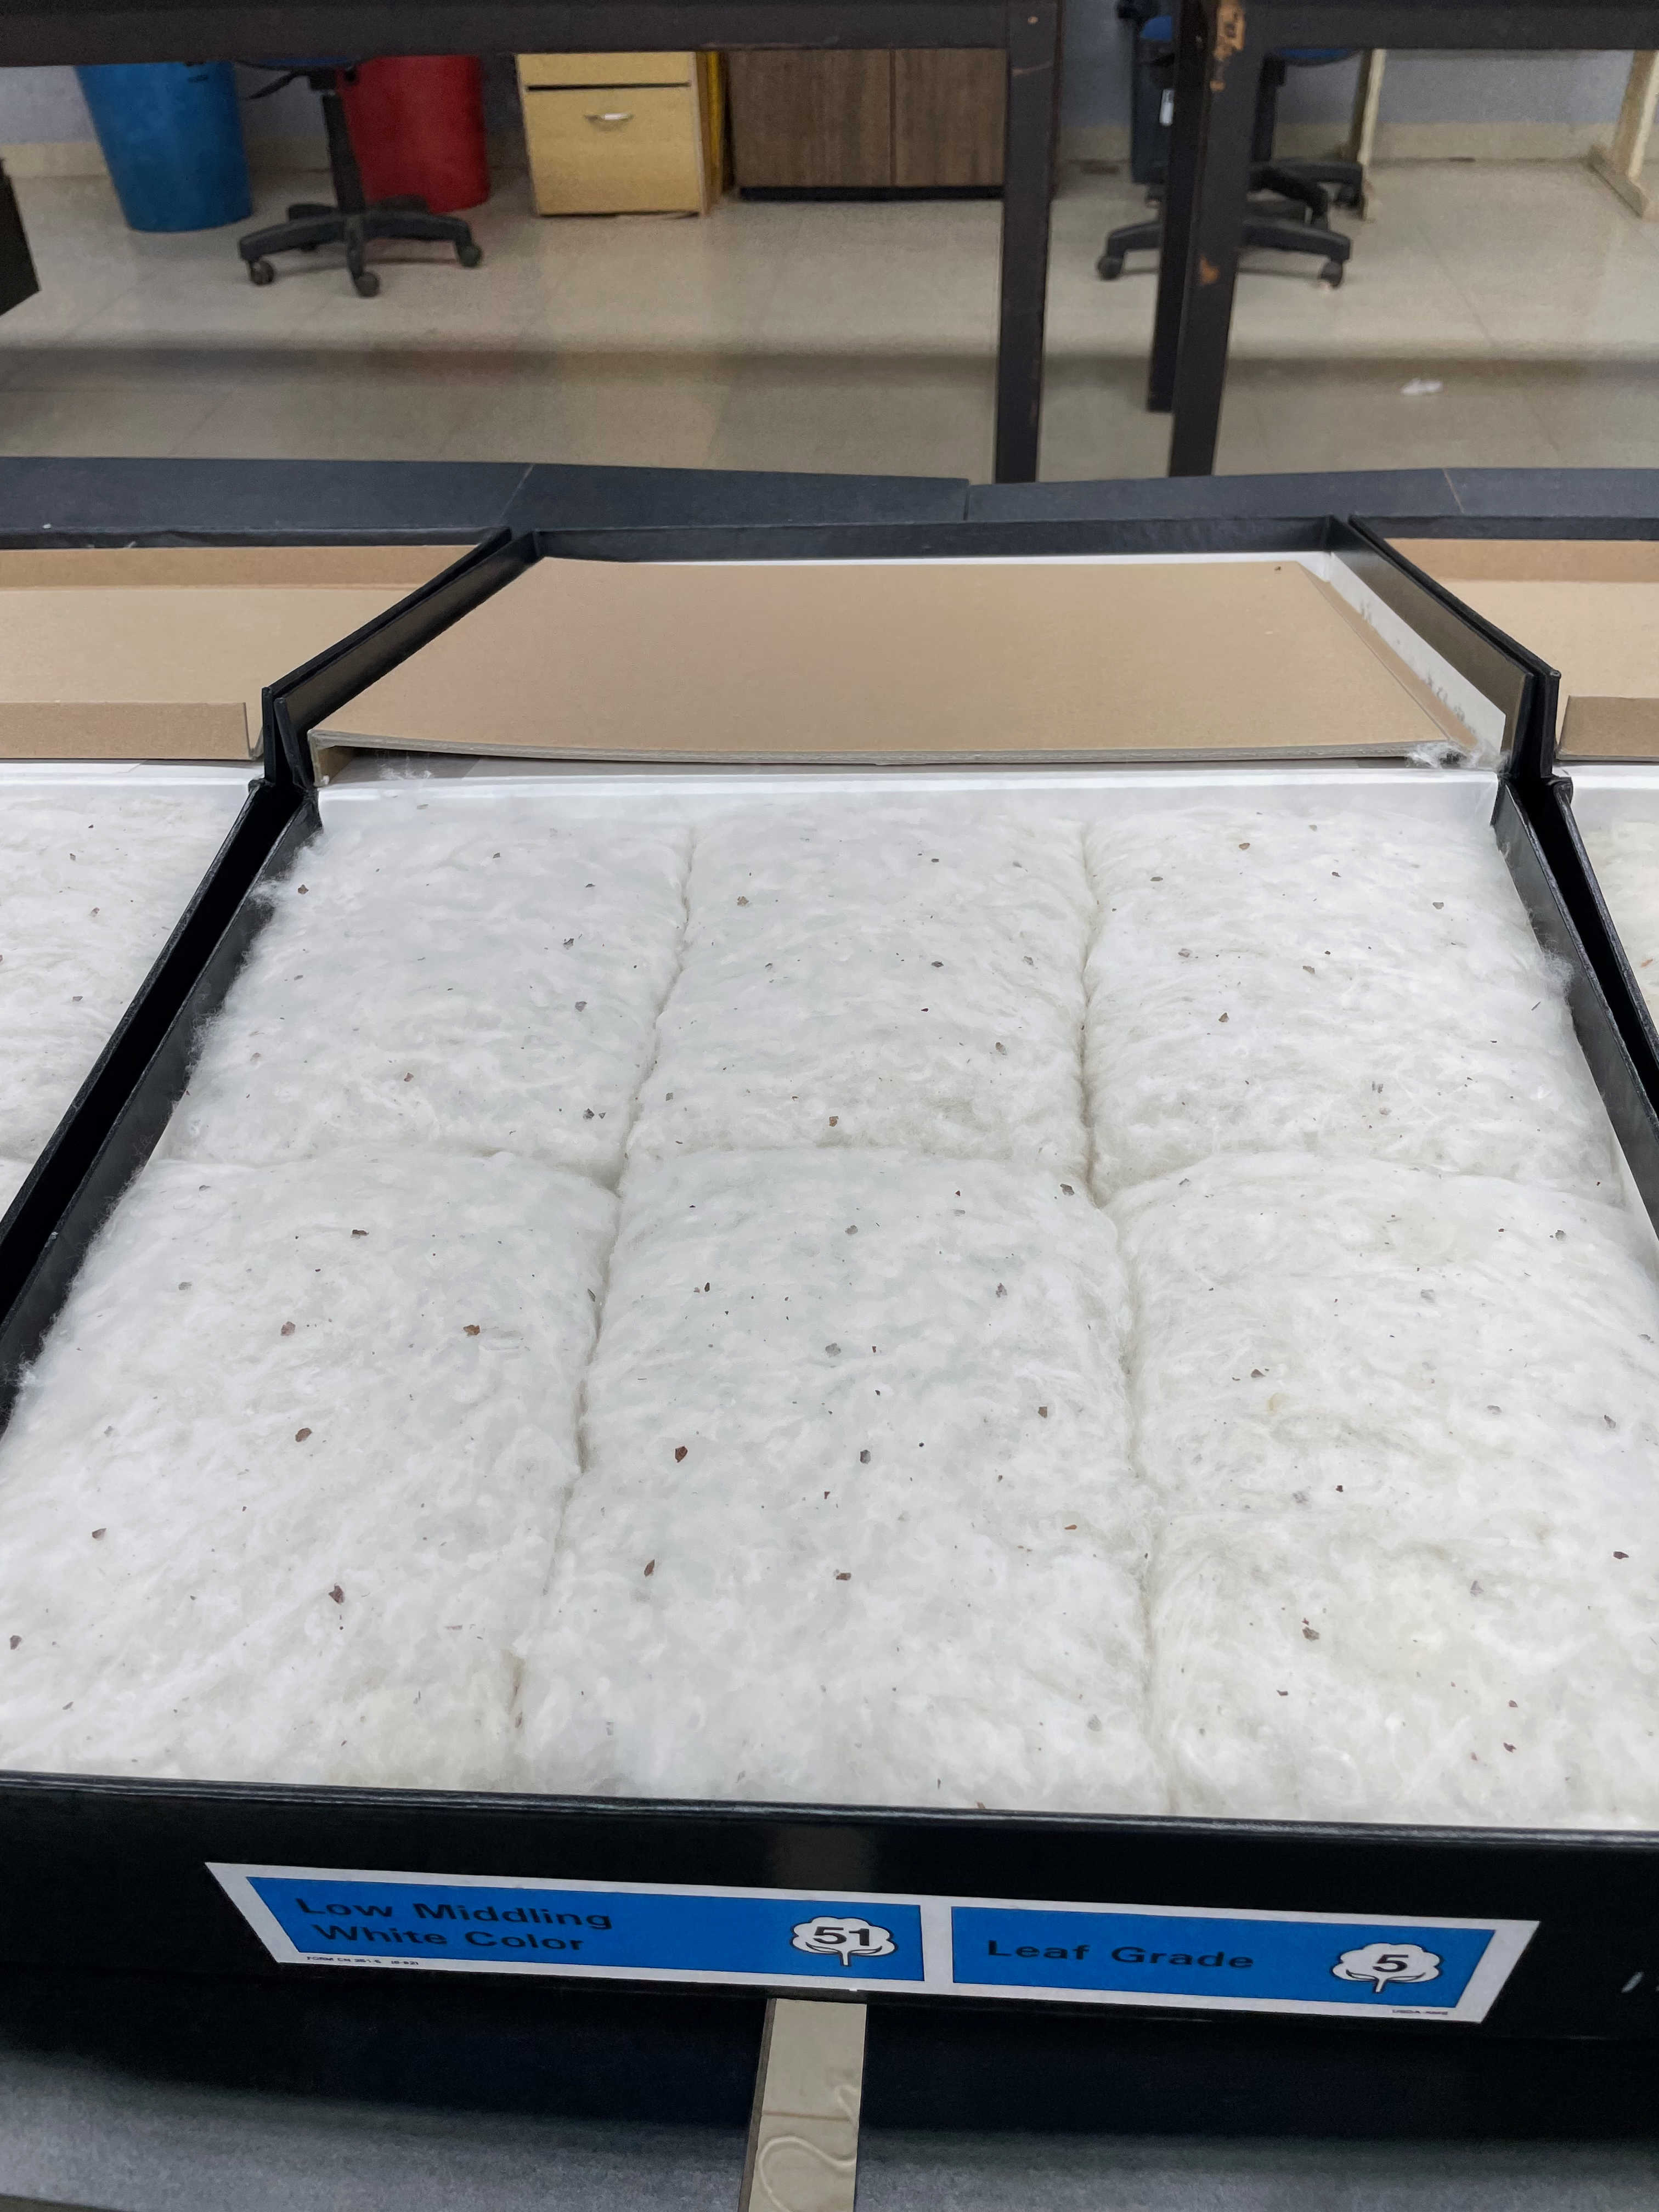
\includegraphics[trim={0 0 0 5cm},clip, scale=.3]{images/padrao_fisico_universal.jpeg}
            \end{center}
            \legend{Fonte: Do Autor}
        \end{figure}

        O protocolo de análise é rigoroso e inicia-se pela calibração visual do técnico, que deve memorizar os padrões físicos antes de iniciar a classificação, podendo consultá-los sempre que necessário para evitar desvios de julgamento. O manuseio da amostra exige técnica específica: ela deve ser subdividida longitudinalmente em camadas, com cuidado para não descaracterizar sua estrutura. As duas faces com maior incidência de defeitos visíveis, são selecionadas e voltadas para cima para a avaliação final.

        Neste exame, o classificador julga simultaneamente múltiplos atributos qualitativos, conforme detalhado por \citeonline{abbade2014agro}:

        \begin{itemize}
            \item \textbf{Cor:} Avaliada pela combinação de matiz, saturação e brilho, sendo categorizada em classes (Branco, Ligeiramente Manchado, Manchado, Tingido e Amarelo);
            \item \textbf{Impurezas (Leaf Grade):} Quantificação visual de cascas, folhas, caules e outras matérias estranhas. O grau é atribuído em uma escala de 1 a 8, na qual 1 representa a amostra mais limpa e 8, a mais suja;
            \item \textbf{Preparação:} Identificação de defeitos oriundos do processo de beneficiamento, como a aspereza e a formação de nós de fibra (emaranhados de fibras);
            \item \textbf{Contaminações:} Presença de materiais não vegetais (plásticos, óleos, entre outros) que desclassificam o lote.
        \end{itemize}

        A determinação final do ``Tipo'' é uma composição entre o padrão de cor e o grau de folha, registrada no Laudo de Classificação (Tabela \ref{tab_tipo_cor}).

        Apesar da padronização dos critérios, a classificação visual possui limitações inerentes à percepção humana. \citeonline{matusiak2010important} argumentam que a análise sensorial é fortemente influenciada por fatores como cansaço visual, experiência do técnico e condições de iluminação. Essa subjetividade gera variabilidade nos resultados, tanto entre diferentes avaliadores quanto nas decisões do mesmo técnico em momentos distintos. Além disso, a dificuldade natural do olho humano em distinguir nuances sutis de cor ou quantificar impurezas milimétricas reforça a necessidade de sistemas de Visão Computacional, que oferecem a reprodutibilidade e a precisão objetiva exigidas pela indústria.

        \afterpage{%
    \clearpage% Flush earlier floats (otherwise order might not be correct)
    \thispagestyle{empty}% empty page style (?)
    \begin{landscape}% Landscape page
        \centering % Center table
        \begin{table}
            \centering
            \caption{Códigos dos tipos de Cor, Classes de Cor ou Grau de Cor do Algodão Upland}
            \begin{tblr}{
                width = \linewidth,
                colspec = {Q[l,m,400]Q[c,m,180]Q[c,m,220]Q[c,m,180]Q[c,m,220]Q[c,m,180]},
                row{1} = {font=\bfseries},
                vline{2-6} = {-}{},
                hline{3-9} = {-}{},
                hline{1-2,10} = {2pt}
              }
                                                                                  & Branco & Ligeiramente Creme & Creme & Avermelhado & Amarelado \\
              Cor Boa Média - GM (Good Middling)                         & 11              & 12                          & 13             & -                    & -                  \\
              Cor Estritamente Média-SM (Strict Middling)                & 21              & 22                          & 23             & 24                   & 25                 \\
              Cor Média-M (Middling)                                     & 31              & 32                          & 33             & 34                   & 35                 \\
              Cor Estritamente Abaixo da Média-SLM (Strict Low Middling) & 41              & 42                          & 43             & 44                   & -                  \\
              Cor Abaixo da Média-LM (Low Middling)                      & 51              & 52                          & 53             & 54                   & -                  \\
              Cor Estritamente Boa Comum-SGO (Strict Good Ordinary)      & 61              & 62                          & 63             & -                    & -                  \\
              Cor Boa Comum-GO (Good Ordinary)                           & 71              & -                           & -              & -                    & -                  \\
              Abaixo de Padrão                                           & 81              & 82                          & 83             & 84                   & 85                 
              \end{tblr}
        \label{tab_tipo_cor}
        \end{table}
    \end{landscape}
    \clearpage
}

    \subsubsection{O Impacto do Viés Subjetivo Humano na Definição do Padrão de Referência (\textit{Ground Truth})}
    \label{sec:vies_humano_gt}

        A qualidade preditiva de qualquer sistema de visão computacional profundo é intrinsecamente
        limitada pela fidelidade do sinal de rotulagem utilizado como padrão de referência
        (\textit{ground truth}). Para além dos fatores já discutidos --- cansaço visual, experiência
        do técnico e condições de iluminação --- a subjetividade da tipagem visual regida pela
        Instrução Normativa nº 24/2016 do MAPA é também influenciada por um viés cognitivo-comercial
        do avaliador, resultando em uma concordância entre classificadores humanos experientes que é
        historicamente instável, tanto entre diferentes avaliadores quanto nas decisões do mesmo
        técnico em momentos distintos \cite{matusiak2010important, fisher2023aiassisted}.

        Uma vez que o conjunto de dados de referência utilizado nesta dissertação foi rotulado a
        partir dos laudos de classificação visual humana da algodoeira parceira em Sapezal, Mato
        Grosso (Seção \ref{sec:conjunto_dados}), as inconsistências inerentes ao julgamento humano
        atuam como um ruído estocástico incorporado aos próprios rótulos de treinamento. Esse fator
        impõe um limite superior (\textit{upper bound}) ao desempenho teórico absoluto das redes
        neurais avaliadas, uma vez que os modelos são forçados a mapear fronteiras de decisão
        qualitativas e fluidas que, por vezes, carecem de consistência física estrita.

        \clearpage

    \subsubsection{A Classificação Instrumental (HVI)}

        Paralelamente à análise visual, a segunda amostra de trabalho é destinada à classificação instrumental. Diferente da avaliação humana, essa etapa exige rigoroso controle ambiental: as amostras devem permanecer em repouso em bandejas teladas por, no mínimo, 24 horas em laboratório climatizado (temperatura e umidade controladas) para atingir o equilíbrio de umidade com o ambiente, garantindo a reprodutibilidade das leituras físicas.

        A análise é realizada em equipamentos de alto volume conhecidos como HVI, calibrados diariamente com padrões internacionais do USDA. A Figura \ref{fig_hvi_maquina} apresenta o modelo Uster HVI 1000, amplamente adotado pela indústria têxtil.

        \begin{figure}[H]
            \caption{\label{fig_hvi_maquina}Equipamento Uster HVI 1000}
            \begin{center}
                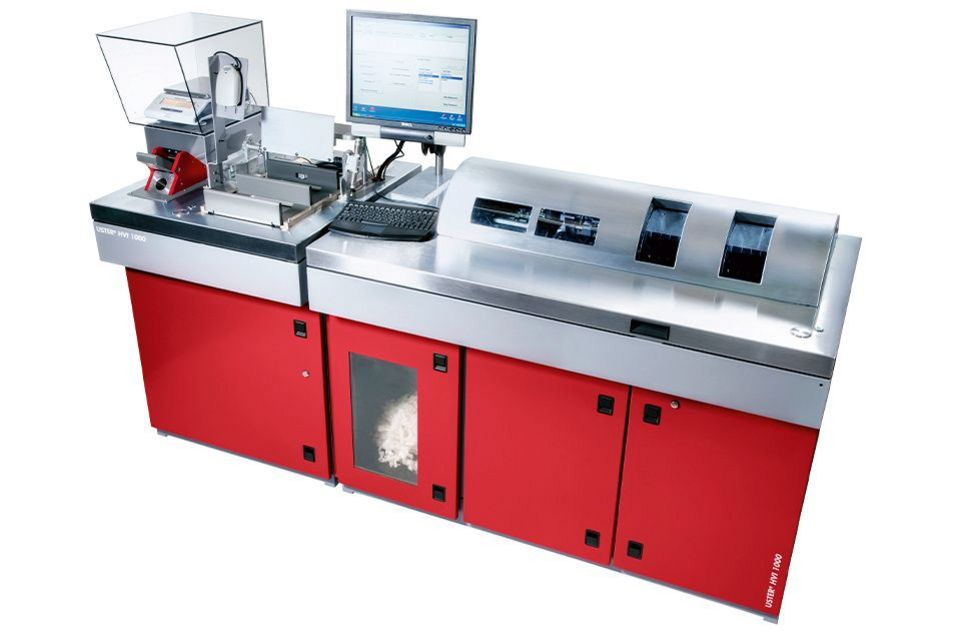
\includegraphics[trim={0 0 0 0},clip, scale=.3]{images/hvi_maquina.jpg}
            \end{center}
            \legend{Fonte: \cite{uster2024hvi}}
        \end{figure}

        O protocolo operacional do HVI automatiza a mensuração de múltiplas propriedades físicas. O teste de \textit{Micronaire} é realizado em um único corpo de prova por meio da compressão de massa de fibras, enquanto os demais parâmetros de comprimento e resistência são obtidos por meio de pentes óticos e garras mecânicas em dois corpos de prova por amostra, gerando uma média do lote.

        Os principais parâmetros fornecidos no laudo técnico são:

        \begin{itemize}
            \item \textbf{Comprimento da Fibra (UHML):} Comprimento médio da metade superior das fibras.
            \item \textbf{Índice de Uniformidade do Comprimento da Fibra (\%UI):} Relação entre o comprimento médio total das fibras e o comprimento médio das fibras mais longas.
            \item \textbf{Resistência ou Tenacidade da Fibra (Str):} Medida da força necessária para romper as fibras, expressa em gf/tex.
            \item \textbf{Alongamento à Rotura da Fibra (\%Elg):} Percentual de extensão que a fibra suporta antes de romper.
            \item \textbf{Micronaire da Fibra (Mic):} Combinação de finura e maturidade da fibra.
            \item \textbf{Grau de Reflectância (\%Rd):} Nível de luminosidade e cor branca refletida pelas fibras.
            \item \textbf{Grau de Amarelamento (+b):} Índice que expressa o nível de amarelamento da fibra.
            \item \textbf{Índice de Fibras Curtas (\%SFI):} Percentual de fibras com comprimento inferior a 0,50 polegadas.
            \item \textbf{Índice de Consistência da Fiação (SCI):} Valor calculado com base nas propriedades físicas das fibras e sua correlação com a performance de fiação.
        \end{itemize}

        Embora o HVI tenha trazido objetividade às transações comerciais, ele apresenta limitações críticas sob a ótica da classificação final. Além do alto custo de aquisição e manutenção \cite{cottonbrazil2021}, o equipamento fornece métricas baseadas em médias globais da amostra. Isso significa que, embora o HVI quantifique com precisão a área total de impurezas, ele não captura a percepção visual holística, como a distribuição espacial da sujeira, a textura e o contraste com a fibra, utilizada pelos classificadores humanos para determinar o ``Tipo'' comercial. Essa lacuna de percepção é justamente o nicho onde sistemas de visão computacional baseados em aprendizado profundo se destacam, pois são capazes de correlacionar padrões visuais complexos diretamente com os graus de qualidade padronizados, oferecendo uma alternativa automatizada e consistente à subjetividade humana.

    \subsubsection{A Relação entre o Visual e o Instrumental}

        A integração entre a subjetividade da análise visual e a objetividade instrumental baseia-se historicamente nos estudos de \citeonline{nickerson1958grade}. Buscando traduzir a percepção humana para grandezas físicas mensuráveis, os autores desenvolveram o colorímetro Nickerson-Hunter, estabelecendo as bases para o atual diagrama de cores utilizado pelo sistema HVI.

        Conforme ilustrado na Figura \ref{fig_hvi_color_chart}, a relação é estabelecida em um plano bidimensional no qual:

        \begin{itemize}
            \item O eixo vertical (\textbf{\%Rd}) representa a \textbf{Reflectância} (brilho), correlacionando-se com a escala de cinzas (do branco ao cinza escuro);
            \item O eixo horizontal (\textbf{+b}) representa o \textbf{Grau de Amarelamento}, indicando a saturação da cor amarela na fibra.
        \end{itemize}

        As interseções desses valores formam clusters que correspondem às classes visuais tradicionais (por exemplo, \textit{Middling}, \textit{Strict Low Middling}). Dessa forma, o HVI consegue converter leituras sensoriais em uma ``nota'' comercial compatível com o julgamento humano.

        \clearpage
        \begin{figure}[H]
            \caption{\label{fig_hvi_color_chart}Diagrama de Cores relacionando parâmetros físicos (\%Rd e +b) com a classificação visual.}
            \begin{center}
                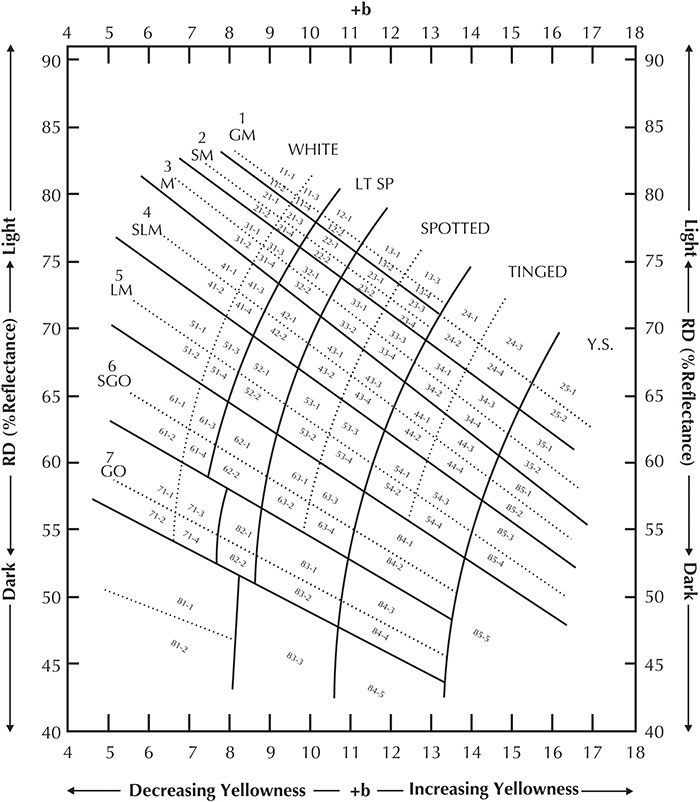
\includegraphics[trim={0 0 0 0},clip, scale=.5]{images/hvi_color_chart.jpg}
            \end{center}
            \legend{Fonte: \citeonline{cottoninc2024hvicolor}}
            % \nota{}
        \end{figure}

        Entretanto, essa correlação robusta observada na análise de cor não se verifica com a mesma eficácia para os parâmetros de impurezas e preparação. Enquanto o HVI mensura a sujeira por contagem de partículas e área ocupada, o classificador humano avalia a aparência geral, considerando o contraste, o tamanho e a natureza do resíduo (folha, casca ou caule). Estudos indicam que a correlação entre o ``Grau de Folha'' visual e a leitura de ``\%Area'' do HVI pode ser baixa em lotes com sujeira heterogênea.

        Essa discrepância evidencia uma lacuna tecnológica: o instrumento é preciso na física (cor), mas limitado na interpretação de padrões complexos (sujeira e textura). É nesse cenário que se insere a proposta desta dissertação: utilizar técnicas de visão computacional para reproduzir a percepção cognitiva humana, buscando uma classificação de qualidade que considere não apenas a estatística da sujeira, mas sua morfologia e distribuição visual na pluma.


\section{Visão Computacional Aplicada à Agricultura}
\label{sec:cv_agricultura}

    Esta seção explora os fundamentos teóricos da visão computacional e dos sistemas de processamento de imagens. A partir de um resgate histórico da disciplina, o texto detalha a arquitetura formal desses sistemas e sua aplicação no agronegócio, com ênfase nas tecnologias e métodos aplicados à cultura do algodão.

    A visão computacional, embora frequentemente associada às inovações recentes da inteligência artificial, possui raízes que remontam a meados do século XX. Segundo a revisão histórica de \citeonline{oliveira2024visao}, a área foi idealizada inicialmente em 1955, sob a premissa de equipar computadores com capacidades sensoriais análogas aos ``olhos e ouvidos'' humanos. Nas décadas seguintes, especialmente nos anos 1970, pesquisadores acreditavam que a emulação da visão biológica seria um marco rapidamente alcançável. Nesse contexto, destaca-se o trabalho seminal de \citeonline{marr1976vision} no campo da neurofisiologia, que propôs uma abordagem computacional para a visão, formulando algoritmos para a interpretação de cenas que serviram como alicerce para grande parte da pesquisa subsequente \cite{vaina2004marr}.

    Contudo, a evolução da área revelou que o processamento visual era intrinsecamente mais complexo do que o previsto, dada a lacuna de conhecimento sobre como o próprio cérebro humano interpreta estímulos visuais. Após décadas de avanços progressivos e o aumento do poder computacional, a visão computacional consolidou-se como a disciplina científica dedicada ao desenvolvimento de métodos que permitem às máquinas não apenas capturar, mas interpretar e ``compreender'' imagens com um nível de abstração semelhante à percepção humana \cite{ballard1982computer}.

    % Revisado
\subsection{Fundamentos de um Sistema de Visão Computacional}

    Um sistema de visão computacional é a integração de \textit{hardware} e \textit{software} projetada para simular a percepção visual humana. \citeonline{saldana2013review} definem que tais sistemas têm o objetivo de extrair e analisar informações de objetos de forma automática, objetiva e não invasiva. A arquitetura típica estrutura-se de três pilares fundamentais: o dispositivo de aquisição de imagens (sensores), o sistema de iluminação e a unidade de processamento (software).

    \subsubsection{Aquisição de imagens}

        A aquisição da imagem é o primeiro estágio do processo, no qual a radiação eletromagnética refletida pelo objeto é convertida em dados digitais. Embora existam sensores baseados em ultrassom, raios-X e espectroscopia no infravermelho próximo (\textit{Near Infrared} --- NIR), as câmeras digitais operando no espectro visível são os dispositivos predominantes na agricultura de precisão \cite{brosnan2004improving}.

        No núcleo dessas câmeras, a captura é realizada por dois tipos principais de sensores: CCD (\textit{Charge-Coupled Device}) e CMOS (\textit{Complementary Metal-Oxide-Semiconductor}).

        As câmeras CCD são historicamente reconhecidas pela alta fidelidade de imagem e sensibilidade em condições de baixa luminosidade. Isso decorre de sua arquitetura, que privilegia uma maior área fotossensível (fator de preenchimento) e uniformidade na resposta dos pixels, resultando em baixo ruído e ampla faixa dinâmica. Tais características as tornaram padrão em aplicações científicas de alta precisão. Contudo, seu alto consumo energético e a complexidade dos circuitos externos limitam sua portabilidade \cite{littwiller2001ccd_cmos}.

        Em contrapartida, a tecnologia CMOS evoluiu drasticamente nas últimas décadas. Sua arquitetura permite a integração de conversores e amplificadores diretamente no pixel, reduzindo o consumo de energia, o tamanho físico e o custo de fabricação. Embora versões antigas apresentassem maior ruído, sensores CMOS modernos atingiram níveis de qualidade comparáveis aos CCDs, tornando-se a escolha dominante para dispositivos móveis e sistemas embarcados no campo \cite{bigas2006cmos}. O Quadro \ref{quad:ccd_vs_cmos} resume as diferenças técnicas entre as tecnologias.

        \begin{table}[ht]
    \centering
    \caption{Resumo comparativos das principais características entre sensores CCD e CMOS}
    \begin{tabular}{l|c|c}
    \hline
    \textbf{Característica}             & \textbf{CCD}                  & \textbf{CMOS}                  \\ \hline
    Consumo de energia                  & Alto                          & Baixo                          \\ 
    Custo                               & Alto                          & Baixo                          \\ 
    Integração em chip                  & Não                           & Sim                            \\ 
    Flexibilidade                       & Limitada                      & Alta                           \\ 
    Faixa dinâmica                      & Alta                          & Limitada                       \\ 
    Sensibilidade                       & Alta                          & Limitada                       \\ 
    Ruído                               & Baixo                         & Alto                           \\ 
    Qualidade de imagem                 & Alta                          & Limitada                       \\ 
    Velocidade                          & Limitada                      & Alta                           \\ 
    Tamanho físico do sistema           & Maior                         & Menor                          \\ 
    Aplicações                          & Alta qualidade, ciências      & Dispositivos móveis, segurança \\ \hline
    \end{tabular}
    \label{tab:ccd_vs_cmos}
    \legend{Fonte: \citeonline{bigas2006cmos}}
\end{table}

        No entanto, para a aplicação específica da classificação de algodão, a escolha do sensor impõe desafios críticos que vão além da arquitetura de fabricação. A natureza física da pluma exige características sensoriais específicas para garantir a correlação com os padrões comerciais:

    \begin{enumerate}
        \item \textbf{Faixa Dinâmica (\textit{Dynamic Range}):} O algodão beneficiado possui alta refletância (brilho), criando um cenário de alto contraste em que as impurezas são significativamente mais escuras que a fibra. \citeonline{li2025measurement} destacam que a captura de imagens nesse cenário enfrenta o desafio de sombras e brilho excessivo; sensores com baixa faixa dinâmica tendem a saturar nos brancos ou perder detalhes nas áreas sombreadas das impurezas, exigindo algoritmos robustos de segmentação (como o Color-Unet) para garantir a consistência da medição de cor.
        
        \item \textbf{Resolução Espacial:} A detecção de impurezas milimétricas impõe um desafio de amostragem. \citeonline{li2025cottonyolo} argumentam que métodos tradicionais falham em detectar esses pequenos objetos devido à complexidade do fundo e à mistura de pixels. O uso de sensores de alta resolução, aliados a redes neurais profundas, torna-se mandatório para distinguir contaminantes minúsculos que, em resoluções menores, seriam invisíveis ou confundidos com ruído.
        
        \item \textbf{Fidelidade de Cor:} A classificação comercial depende estritamente dos parâmetros de Amarelamento (+b) e Reflectância (Rd). Segundo \citeonline{li2023novel}, a simples captura RGB (\textit{Red, Green, Blue}) não garante a correlação com o padrão HVI. É necessária uma calibração rigorosa e a conversão para espaços de cor perceptuais (como CIE $L^*a^*b^*$ ou Hunter) para que o sistema de visão atinja coeficientes de determinação superiores a 0,88 quando comparado aos colorímetros industriais, evitando erros de graduação que resultam em prejuízo financeiro.
    \end{enumerate}


        Além do sensor, a integridade da análise depende do formato de armazenamento. Em aplicações científicas, formatos de compressão sem perdas, como PNG, BMP ou TIFF, são preferíveis, pois preservam o valor exato de cada pixel. Formatos com perdas, como o popular JPEG, utilizam algoritmos que descartam informações de alta frequência para reduzir o tamanho do arquivo. Para a classificação de algodão, na qual a textura fina e a presença de micro-impurezas são críticas, os artefatos de bloco gerados pela compressão JPEG podem ser interpretados erroneamente pelos algoritmos como ruído ou defeitos, comprometendo a precisão do modelo \cite{vanderwalt2014scikit}.


    \subsubsection{Iluminação}

        A iluminação é um componente crítico nos sistemas de visão computacional, pois define as propriedades ópticas de absorção, reflexão e transmissão dos objetos analisados. Uma captura bem iluminada reduz a necessidade de etapas algorítmicas complexas de pré-processamento, aumentando a eficiência computacional e a precisão das análises \cite{chen2002machine_vision}. Segundo \citeonline{zhang2014computer}, a fonte de luz ideal deve fornecer uma incidência uniforme e estável, realçando as características de interesse e mitigando reflexos ou sombras indesejáveis que possam comprometer a segmentação do objeto.

        No contexto específico da classificação de algodão, a iluminação desempenha um papel duplo e, por vezes, antagônico, exigindo um compromisso técnico (\textit{trade-off}):

        \begin{itemize}
            \item \textbf{Para Análise de Cor (Simulação de HVI):} A classificação comercial baseia-se na reflectância (\%Rd) e no amarelamento (+b). \citeonline{rady2025computervision}, ao desenvolverem sistemas de visão para graduação de algodão egípcio, demonstraram que a consistência na classificação de cor exige uma iluminação difusa e homogênea. O uso de luz direcional cria sombras e reflexos na fibra que alteram os valores RGB capturados, impedindo a correlação direta com os padrões físicos universais.
            
            \item \textbf{Para Detecção de Impurezas e Robustez:} Paradoxalmente, a luz difusa que favorece a cor tende a ``suavizar'' a textura, ocultando defeitos tridimensionais. \citeonline{verma2026graphcotton} destacam que a variabilidade de iluminação é um dos principais desafios para a segmentação robusta de capulhos e impurezas em cenários complexos. Para detectar contaminantes que possuem a mesma cor da fibra (como plásticos claros) ou defeitos de preparação (nós de fibra), uma componente de luz direcional ou rasante é fundamental para gerar microssombras que revelam a morfologia do objeto, permitindo que modelos de detecção superem as limitações da simples análise de cor.
        \end{itemize}

        Atualmente, a tecnologia LED (\textit{Light-Emitting Diode}) consolidou-se como padrão para solucionar esse dilema. Sua estabilidade espectral e capacidade de controle rápido permitem o desenvolvimento de sistemas de iluminação híbridos ou multiespectrais, que alternam entre configurações difusas e direcionais para capturar o máximo de informação da amostra em uma única inspeção \cite{cubero2010advances}.

        Dessa forma, o projeto do sistema de iluminação para esta dissertação não buscou apenas a visibilidade, mas a fidelidade fotométrica, garantindo que a imagem digital servisse como um \textit{proxy} confiável tanto para a avaliação cromática quanto para a inspeção morfológica da qualidade.


    \subsubsection{Software}

        O componente de \textit{software} atua como o cérebro do sistema de visão computacional, responsável não apenas por orquestrar o \textit{hardware} de captura e iluminação, mas principalmente por implementar os algoritmos de interpretação visual. Historicamente, o desenvolvimento baseava-se em bibliotecas de processamento de imagem clássico (ou \textit{rule-based}), como o OpenCV (\textit{Open Source Computer Vision Library}). Essas ferramentas exigiam que o engenheiro definisse manualmente os descritores matemáticos para extrair bordas, cores ou formas geométricas \cite{opencv_library}.

        No entanto, o estado da arte na agricultura de precisão sofreu uma mudança de paradigma com a consolidação do aprendizado profundo (\textit{Deep Learning}). Conforme revisado por \citeonline{mustofa2023comprehensive}, o foco do desenvolvimento de \textit{software} migrou da engenharia de características manual (\textit{feature engineering}) para a curadoria de dados e o treinamento de redes neurais convolucionais (\textit{Convolutional Neural Networks} --- CNNs). Nesse novo cenário, o \textit{software} não segue mais regras lógicas rígidas baseadas em limiares de cor, mas aprende padrões complexos a partir de exemplos, exigindo \textit{frameworks} robustos para o treinamento e inferência dos modelos.

        Atualmente, dois ecossistemas dominam o desenvolvimento de \textit{software} para visão agrícola:

        \begin{itemize}
            \item \textbf{\textit{Frameworks} de Treinamento (PyTorch/TensorFlow):} São as plataformas nas quais os modelos são construídos. Uma revisão recente de \citeonline{zhang2025bibliometric} destaca que, embora o TensorFlow tenha sido pioneiro na produção industrial, o PyTorch ganhou predominância na pesquisa agrícola devido à sua flexibilidade e facilidade de \textit{debugging}, permitindo a prototipagem rápida de novas arquiteturas para diversas aplicações.
            
            \item \textbf{Arquiteturas de Detecção (YOLOv8/Transformers):} O \textit{software} moderno implementa arquiteturas pré-treinadas que oferecem o equilíbrio ideal entre velocidade e precisão. \citeonline{jelali2025improvedyolov8} destacam a arquitetura YOLOv8 (\textit{You Only Look Once}, versão 8) como o padrão atual para monitoramento agrícola em tempo real, superando antecessores na detecção de pequenos objetos em cenários não estruturados, o que representa uma característica vital para identificar impurezas minúsculas no algodão.
        \end{itemize}

        Por fim, uma camada crítica do \textit{software} frequentemente negligenciada é a ferramenta de anotação e gestão de dados. Como a performance do modelo depende estritamente da qualidade dos exemplos fornecidos (``Garbage In, Garbage Out''), o uso de plataformas para rotulagem consistente de imagens tornou-se um pré-requisito. \citeonline{yang2025ip} argumentam que a falta de anotações precisas é hoje o maior gargalo para a aplicação de visão computacional no campo, exigindo softwares que facilitem a marcação semântica de defeitos e o aumento de dados para robustecer o modelo contra variações de iluminação.

\subsection{Processamento e Análise de Imagens}

    O processamento e a análise de imagens constituem o núcleo algorítmico dos sistemas de visão, transformando a matriz numérica bruta capturada pelo sensor em informações semânticas para a tomada de decisão. A literatura clássica, consolidada por \citeonline{gonzalez2017digital}, organiza esse fluxo em uma hierarquia de três níveis: baixo, médio e alto nível. Embora a ascensão do aprendizado profundo (\textit{deep learning}) tenha automatizado a transição entre essas etapas, a compreensão dessa estrutura permanece fundamental para o design de sistemas robustos.

    \subsubsection{Processamento de Baixo Nível: Pré-processamento}
    
        O processamento de baixo nível engloba operações nas quais tanto a entrada quanto a saída são imagens. O objetivo primordial é a melhoria da qualidade visual e a restauração de dados para facilitar as etapas subsequentes. Técnicas comuns incluem a correção radiométrica (uniformização da iluminação), a redução de ruído via filtros espaciais e a correção geométrica de distorções da lente.
        
        No contexto moderno de redes neurais, esta etapa evoluiu para incluir o aumento de dados (\textit{data augmentation}) e a normalização estatística. \citeonline{shorten2019survey} destacam que, para aplicações agrícolas onde a variabilidade de campo é alta, aplicar transformações geométricas e de cor nas imagens de treinamento é crucial para evitar o \textit{overfitting} e garantir que o modelo generalize bem para diferentes condições de iluminação.

    \subsubsection{Processamento de Nível Intermediário: Segmentação e Representação}
    
        Nesse estágio, a operação transita de imagens para atributos. A tarefa central é a segmentação, que visa particionar a imagem em regiões de interesse: no caso do algodão, separar a fibra do fundo e isolar as impurezas.
        
        Abordagens tradicionais baseavam-se em limiarização (\textit{thresholding}) e detecção de bordas \cite{sonka1993}. Contudo, \citeonline{li2025cottonyolo} argumentam que métodos clássicos falham na classificação de algodão devido à complexidade da textura: sombras na fibra podem ser confundidas com sujeira, e impurezas claras (como plásticos) não possuem contraste suficiente para uma limiarização simples.
        
        Essa limitação impulsionou a adoção de redes neurais convolucionais (CNNs). Diferentemente da extração manual de atributos (forma, textura, momentos), as CNNs aprendem hierarquicamente as representações necessárias: as primeiras camadas da rede atuam como filtros de borda e textura, enquanto as camadas profundas agem como segmentadores semânticos, identificando padrões complexos que escapam à modelagem matemática tradicional \cite{lecun2015deep}.

    \subsubsection{Processamento de Alto Nível: Interpretação e Classificação}
    
        O nível final envolve a ``compreensão'' da cena, atribuindo significado aos objetos segmentados. Na classificação de qualidade do algodão, isso não significa apenas detectar uma partícula, mas interpretá-la semanticamente: classificar se é uma folha, um caule ou um defeito de preparação (\textit{nep}) e, com base no conjunto, atribuir uma nota global ao fardo (Tipo/Grau).
        
        Enquanto sistemas antigos utilizavam classificadores estatísticos (como SVM ou KNN) sobre vetores de características fixos, os sistemas modernos realizam a classificação de forma integrada. O modelo aprende a correlacionar a distribuição espacial e morfológica das impurezas diretamente com os padrões de qualidade comercial, emulando o processo cognitivo de um classificador humano experiente \cite{pacal2024systematic}.

\subsection{Aplicações da Visão Computacional}

    A aplicação da visão computacional no agronegócio ultrapassou a fase experimental para se tornar uma ferramenta essencial na garantia de qualidade e produtividade. A literatura recente evidencia uma migração das técnicas clássicas de processamento de imagem para abordagens baseadas em aprendizado profundo, capazes de lidar com a variabilidade natural dos produtos agrícolas \cite{patricio2018,tian2020}.
    
    Na sequência, discute-se como essa tecnologia evoluiu do monitoramento de campo para a rigorosa inspeção de qualidade industrial, nicho no qual este trabalho se insere.

    \subsubsection{Monitoramento e Detecção de Padrões em Campo}

        No ambiente de cultivo, a visão computacional é amplamente utilizada para a detecção de anomalias biológicas. \citeonline{ahad2023} e \citeonline{ritharson2023} demonstraram que CNNs podem superar a sensibilidade humana na identificação de doenças, atingindo níveis de acurácia superiores a 98\% em culturas de arroz. A tendência atual é a implementação desses modelos em arquiteturas leves (como YOLOv8) para processamento em tempo real \cite{shwetha2024}.
        
        Essa capacidade de detecção estende-se à cultura do algodão ainda no campo. \citeonline{singh2023}, por exemplo, desenvolveram algoritmos para identificar capulhos maduros em tempo real, buscando a automação da colheita. Embora a detecção em campo esteja avançada, o maior desafio tecnológico reside na etapa seguinte: a avaliação da qualidade do produto colhido.

    \subsubsection{Inspeção de Qualidade e Padronização Pós-Colheita}

        A avaliação de qualidade de produtos agrícolas, historicamente subjetiva, tem sido transformada pela automação visual. Desde os trabalhos pioneiros de \citeonline{Majumdar1999} na classificação de cereais por textura, a tecnologia evoluiu para detectar defeitos sutis, muitas vezes imperceptíveis ao olho humano, em esteiras de alta velocidade. \citeonline{zhu2024} aplicaram técnicas de luz estruturada para identificar danos mecânicos em maçãs, validando o uso de visão computacional para a tipificação comercial.

        No contexto específico da fibra de algodão, a pureza e a cor são os atributos mais críticos. A detecção de contaminantes (\textit{foreign matter}) é um problema clássico revisitado por \citeonline{wang2023}, que implementaram a arquitetura YOLOv5 para distinguir fibras de materiais estranhos (cascas, plásticos) com alta velocidade. A complexidade desta tarefa assemelha-se à detecção de ervas daninhas em campo, na qual a distinção entre o ``alvo'' e o ``fundo'' exige robustez contra variações de iluminação e oclusão \cite{juwono2023, subeesh2022}.
        
        Apesar desses avanços pontuais na detecção de contaminantes, ainda existe uma lacuna na correlação direta entre os padrões visuais aprendidos por máquinas e as classes comerciais manuais (Tipo e Cor) utilizadas na comercialização da pluma, conforme estabelecido pelos Padrões Universais. É nessa intersecção entre a avançada capacidade de detecção de objetos (YOLO/CNNs) e a necessidade de padronização comercial que esta dissertação atua.

\section{Classificação Automatizada do Algodão com Visão Computacional}
\label{sec:classificacao_algodao}

    A classificação da pluma de algodão, historicamente dependente da inspeção manual ou de instrumentos laboratoriais como o HVI, atravessa uma profunda mudança de paradigma impulsionada pela inteligência artificial. A convergência entre processamento de imagem, aprendizado de máquina e tecnologias conectadas (\textit{IoT/Edge Computing}) tem se consolidado como uma solução transformadora para superar as limitações dos métodos tradicionais, que frequentemente exigem mão de obra intensiva, demandam tempo excessivo e estão sujeitos à subjetividade.

    A literatura recente evidencia que a aplicação dessas tecnologias evoluiu substancialmente, expandindo-se do monitoramento agrícola em campo para a automação rigorosa do ``processamento inteligente'' e da inspeção de qualidade na indústria. O uso do aprendizado profundo assumiu um papel dominante nesse cenário, viabilizando a extração de características complexas da fibra que abordagens matemáticas ou estatísticas convencionais não conseguiam modelar com precisão.

    Esta seção explora a trajetória tecnológica dessa automação, abordando desde as limitações físicas dos sensores de captura até a evolução dos modelos preditivos. A discussão abrange a transição do aprendizado de máquina clássico para o atual estado da arte baseado em redes neurais convolucionais e transformers, detalhando como a pesquisa moderna tem solucionado a avaliação automatizada dos três pilares da qualidade comercial do fardo: cor, impurezas (\textit{trash}) e preparação.

    %Revisado
\subsection{Limitações Sensoriais e Multiespectrais}

    Embora câmeras RGB sejam predominantes devido ao baixo custo, a literatura aponta limitações físicas críticas na detecção de certos contaminantes. \citeonline{mustafic2016} demonstraram que materiais como plásticos transparentes e papéis brancos possuem assinaturas visuais quase idênticas à da fibra de algodão no espectro visível, tornando-os virtualmente invisíveis para sensores convencionais. A solução proposta pelos autores envolve o uso de imageamento hiperespectral de fluorescência (UV), capaz de distinguir a composição química de contaminantes não botânicos com precisão superior a 90\%.

    Paralelamente, \citeonline{li2024cottonnet} exploraram o uso de espectroscopia no infravermelho próximo (NIR) combinada com redes neurais (\textit{Cotton-Net}) para estimar o teor de impurezas. Embora o método seja eficaz para determinar a composição química global da amostra, ele carece de informação espacial detalhada para classificar a morfologia dos defeitos, reafirmando a necessidade da visão computacional para a avaliação física do aspecto visual do fardo.

\subsection{O Aprendizado de Máquina e a Variabilidade Intra-Amostra}

    A transição da estatística clássica para o aprendizado de máquina marcou a primeira etapa da automação robusta. \citeonline{fisher2023} investigaram a classificação de algodão egípcio utilizando algoritmos de \textit{Random Forest}, superando abordagens baseadas em Máquinas de Vetores de Suporte (\textit{Support Vector Machines}) e redes neurais artificiais clássicas. Uma contribuição fundamental desse estudo foi a introdução da variância intra-amostra como preditor de qualidade: os autores provaram que a uniformidade da cor ao longo da superfície da amostra é tão determinante para a classificação comercial quanto a média dos valores de reflectância.

    Contudo, a eficácia desses modelos esbarra em um gargalo humano: a qualidade da rotulagem dos dados (\textit{ground truth}). \citeonline{fisher2023aiassisted} alertam que a subjetividade e a fadiga dos classificadores humanos introduzem ruído nos dados de treinamento. Para mitigar o alto custo e a inconsistência da anotação manual, os autores propuseram o uso de aprendizado ativo (\textit{Active Learning}), no qual o sistema solicita intervenção humana apenas para imagens de alta incerteza, reduzindo drasticamente o volume de dados necessários enquanto mantém a acurácia do modelo.

\subsection{Abordagens Contemporâneas de Visão Computacional para o Algodão}

    Atualmente, a fronteira do conhecimento reside na aplicação de CNNs para tarefas de segmentação semântica e detecção de objetos, com foco na correlação direta com os parâmetros do HVI.

    No que tange à análise de cor, o principal desafio é a interferência de sombras e sujeira na leitura dos pixels. \citeonline{li2025measurement} propuseram o método inovador \textit{Color-Unet}. Diferentemente das abordagens que calculam a média de toda a imagem, essa rede realiza a segmentação semântica para isolar a fibra pura, excluindo pixels de impurezas e áreas sombreadas. A medição de cor realizada apenas na máscara de fibra limpa resultou em uma correlação significativamente maior com os valores de referência do HVI.

    Para a detecção de impurezas (\textit{Trash}), a arquitetura YOLO (\textit{You Only Look Once}) estabeleceu-se como padrão. \citeonline{li2025cottonyolo} desenvolveram o modelo \textit{Cotton-YOLO}, uma versão otimizada com módulos de atenção projetados especificamente para detectar impurezas milimétricas que redes genéricas não conseguem identificar. Avançando para a quantificação precisa, \citeonline{jiang2024cottonyoloseg} introduziram o \textit{Cotton-YOLO-Seg}, que não apenas detecta o objeto, mas realiza a segmentação de instância (pixel a pixel). Isso permite o cálculo exato da área ocupada por cada partícula, viabilizando a automação do parâmetro \textit{\% Area} do HVI com precisão inédita.

    Por fim, a avaliação da preparação (irregularidades como nós de fibra) também se beneficia dessas arquiteturas. \citeonline{arachchi2024classification} aplicaram CNNs baseadas em \textit{transfer learning} (como a \textit{Inception V3}) para classificar defeitos em fios de algodão, demonstrando que padrões morfológicos sutis de emaranhamento podem ser aprendidos eficazmente por redes profundas, uma lógica que se estende à avaliação da pluma crua.

\section{Arquiteturas de Aprendizado Profundo para Classificação de Imagens}
\label{sec:arquiteturas}

    A eficácia dos sistemas de visão computacional não está apenas no volume de dados ou no poder de processamento bruto, mas fundamentalmente no \textit{design} das arquiteturas de extração de características. Na classificação da pluma de algodão, o modelo enfrenta um desafio multiescala crônico, exigindo um campo receptivo global para avaliar a uniformidade da cor e a distribuição das fibras, ao mesmo tempo em que necessita de altíssima sensibilidade local para detectar impurezas milimétricas e defeitos de preparação (nós de fibra).

    Historicamente, a superação desses desafios acompanhou a própria evolução das topologias de redes neurais. A transição de redes rasas para modelos ultraprofundos exigiu inovações matemáticas substanciais para lidar com gargalos computacionais e com a degradação do gradiente (\textit{vanishing gradient}). Mais recentemente, a hegemonia das operações puramente convolucionais passou a ser desafiada por mecanismos de autoatenção (\textit{self-attention}) global, redefinindo os limites da representação visual das máquinas.

    Esta seção mapeia a trajetória evolutiva das arquiteturas de estado da arte em classificação de imagens, agrupando-as por seus paradigmas fundamentais de \textit{design}. A análise parte dos blocos construtivos clássicos e da consolidação da profundidade (VGG e Inception), avança pelas soluções de roteamento de gradiente (ResNet e DenseNet), explora os limites da eficiência convolucional (EfficientNet e ConvNeXt) e culmina nos modernos paradigmas baseados em atenção (Vision Transformers e Swin-T). Para cada arquitetura, discute-se não apenas sua inovação teórica, mas principalmente sua viabilidade geométrica e computacional frente à complexidade textural do algodão.

    %Revisado
\subsection{Arquiteturas Fundacionais: VGG e Inception}

    A VGG estabeleceu o uso sistemático de filtros $3 \times 3$, demonstrando que a profundidade é o componente chave para a extração de hierarquias de características. Embora fundamental, sua ineficiência paramétrica e o uso de camadas densas massivas servem hoje como \textit{baseline} histórico. A família Inception introduziu a ideia de processamento multiescala paralelo, capturando texturas em diferentes frequências espaciais, o que pavimentou o caminho para redes com campos receptivos mais inteligentes.

    \subsubsection{A Arquitetura VGG Net}

        A VGG Net, introduzida por \citeonline{vgg2024}, demonstrou que uma rede mais profunda, aliada a uma estrutura uniforme, é o fator determinante para a extração de características em larga escala. Diferentemente de sua predecessora, a \textit{AlexNet}, que utilizava filtros heterogêneos (como $11 \times 11$), a VGG propôs uma filosofia de \textit{design} baseada na simplicidade: a utilização exclusiva de filtros pequenos de $3 \times 3$ empilhados. Matematicamente, uma sequência de três dessas convoluções possui o mesmo campo receptivo efetivo de uma única camada de $7 \times 7$. No entanto, essa abordagem oferece vantagens críticas para a classificação de microtexturas.

        Primeiramente, as três camadas introduzem três funções de ativação ReLU em vez de uma, permitindo que a rede aprenda funções de decisão muito mais complexas e discriminativas. Além disso, enquanto uma camada de $7 \times 7$ com $C$ canais possui $49C^2$ parâmetros, a pilha de três camadas de $3 \times 3$ utiliza apenas $27C^2$ parâmetros. Essa redução de quase 45\% permitiu o aumento da profundidade da rede (até 16 ou 19 camadas) sem um crescimento proibitivo do custo computacional.
        
        Embora existam diversas variantes (de VGG-11 a VGG-19), a VGG-16 tornou-se o padrão para tarefas de visão computacional. Sua estrutura é composta por blocos de camadas convolucionais seguidos por \textit{max-pooling} ($2 \times 2$ com \textit{stride} 2), culminando em camadas totalmente conectadas.

        % \begin{table}[ht]
\centering
\caption{Comparativo Técnico das Arquiteturas VGG Net}
\label{tab:vgg_comparativo}
\begin{tabular}{@{}lccc p{6cm}@{}}
\toprule
\textbf{Modelo} & \textbf{Camadas} & \textbf{Parâmetros} & \textbf{Tamanho (MB)} & \textbf{Diferencial Técnico} \\ \midrule
VGG-11 & 11 & 133M & ~507 & Configuração base; profundidade mínima para convergência. \\
VGG-13 & 13 & 133M & ~508 & Adição de blocos convolucionais duplos no início da rede. \\
VGG-16 & 16 & 138M & ~528 & Equilíbrio ideal entre profundidade e custo; arquitetura SOTA em 2014. \\
VGG-19 & 19 & 144M & ~574 & Máxima capacidade de extração linear; maior custo computacional. \\ \bottomrule
\end{tabular}
\end{table}
        
        Apesar de sua clareza arquitetural, a VGG apresenta limitações em cenários modernos de produção. A dependência de camadas totalmente conectadas massivas resulta em um alto consumo de memória (~528 MB para a VGG-16). Além disso, a ausência de conexões de salto torna o modelo sensível ao desaparecimento do gradiente em profundidades maiores.

        No contexto desta dissertação, a VGG-16 é analisada como um extrator de características robusto. Sua capacidade de capturar microtexturas e sua uniformidade a tornam uma base ideal para \textit{transfer learning}, embora sua eficiência computacional seja inferior a modelos mais recentes como a \textit{EfficientNet}, um ponto crítico para a viabilidade em ambientes agrícolas embarcados.

    \subsubsection{A Arquitetura Inception}

        Enquanto a VGG focava na profundidade linear, a arquitetura Inception (GoogLeNet), introduzida por \citeonline{szegedy2015goingdeeper}, propôs uma mudança arquitetural baseada na esparsidade e na eficiência computacional. O objetivo central era aumentar o poder de representação da rede sem um crescimento paramétrico proibitivo, utilizando para isso o módulo Inception.

        A inovação técnica fundamental da Inception v1 foi o processamento multiescala simultâneo. Em vez de selecionar um tamanho de filtro fixo por camada, o módulo executa convoluções de $1 \times 1$, $3 \times 3$ e $5 \times 5$ em paralelo, concatenando seus resultados. Essa captura multirresolução é altamente vantajosa para a classificação de plumas de algodão: o filtro $3 \times 3$ foca em características locais (fibras individuais e micro-impurezas), enquanto o $5 \times 5$ captura padrões globais (a morfologia geral da amostra). Para viabilizar o custo computacional desse paralelismo, a Inception introduziu convoluções de $1 \times 1$ antes dos filtros maiores para reduzir a profundidade dos canais (\textit{bottleneck}), mantendo a rede leve com 6,8 milhões de parâmetros na v1 (contra 138 milhões da VGG-16).

        As versões subsequentes (v2 e v3) refinaram a arquitetura por meio de princípios de fatoração. Seguindo o objetivo de eficiência matemática, \textit{kernels} grandes ($5 \times 5$) foram substituídos por sequências de $3 \times 3$. Além disso, convoluções quadradas $n \times n$ foram fatoradas em operações assimétricas de $1 \times n$ e $n \times 1$ (ex.: $1 \times 7$ seguido de $7 \times 1$), reduzindo drasticamente as operações em ponto flutuante sem perda de campo receptivo. 

        Esse paradigma de fatoração foi levado ao limite na Xception (\textit{Extreme Inception}) \cite{chollet2017xception}. Essa arquitetura utiliza convoluções separáveis em profundidade (\textit{depthwise separable convolutions}), isolando totalmente a busca por correlações espaciais das correlações entre canais. Dada a sua eficiência paramétrica, consolidou-se como uma das arquiteturas base mais eficazes para tarefas que exigem alta precisão em texturas finas.

        % \begin{table}[ht]
\centering
\caption{Evolução Cronológica e Inovações da Família Inception}
\label{tab:inception_evolution}
\begin{tabular}{@{}ll p{8cm}@{}}
\toprule
\textbf{Versão} & \textbf{Inovação Principal} & \textbf{Impacto Acadêmico / Técnico} \\ \midrule
Inception v1 & Módulo Inception & Introdução do processamento multiescala paralelo e redução de parâmetros. \\
Inception v2 & Batch Normalization & Estabilização do treinamento e aceleração da convergência. \\
Inception v3 & Fatoração Assimétrica & Substituição de filtros $n \times n$ por $1 \times n$ e $n \times 1$; redução de gargalos. \\
Inception v4 & Inception-ResNet & Integração de conexões residuais para treinamento de redes ultra-profundas. \\
Xception & Depthwise Separable & Desacoplamento total de correlações espaciais e de canal; máxima eficiência. \\ \bottomrule
\end{tabular}
\end{table}


\subsection{Conexões Residuais e Densas: ResNet e DenseNet}

    Conforme discutido na seção anterior, avanço na profundidade das redes neurais esbarrou em uma limitação matemática: o problema do desaparecimento do gradiente (\textit{vanishing gradient}). Para solucionar esse gargalo e viabilizar o treinamento de arquiteturas com dezenas ou centenas de camadas, uma nova geração de modelos alterou fundamentalmente o roteamento do fluxo de informações.

    No contexto da classificação de plumas de algodão, essas abordagens tornaram-se essenciais, pois garantem que os detalhes sutis das micro-impurezas não sejam degradados ou perdidos ao longo de um processamento profundo. As subseções a seguir detalham as duas topologias mais influentes dessa fase: a ResNet e a DenseNet.

    \subsubsection{A Arquitetura ResNet}

        A introdução das Redes Residuais (ResNet) por \citeonline{he2016resnet} marcou um ponto de inflexão na visão computacional ao solucionar o problema da degradação em redes ultraprofundas. Antes da ResNet, adicionar camadas a uma CNN resultava em maiores erros de treinamento, devido à dificuldade dos otimizadores em convergir para mapeamentos de identidade em arquiteturas puramente sequenciais.

        Para contornar esse obstáculo, a ResNet fundamenta-se na premissa de que é matematicamente mais eficiente otimizar um resíduo do que um mapeamento direto não referenciado. Em vez de forçar um bloco de camadas a aprender uma função desejada $H(x)$, a arquitetura o restringe a aprender a função residual $F(x)=H(x)-x$. A saída do bloco passa a ser a soma do resíduo com a entrada original, expressa por:
        
        $$H(x)=F(x)+x$$
        
        Essa formulação é materializada na rede por meio de conexões de salto (\textit{skip connections}), atalhos que permitem ao sinal do gradiente fluir pelas camadas sem atenuação. Na classificação de plumas de algodão, em que sutilezas de textura e coloração poderiam ser perdidas por muitas operações de convolução, o caminho de identidade assegura que as características visuais em baixo nível continuem inalteradas até as camadas de decisão.

        A topologia interna da rede adapta-se em função da profundidade desejada, apoiando-se em dois projetos fundamentais de blocos residuais. Para redes de profundidade intermediária (como ResNet-18 e ResNet-34), utiliza-se o bloco básico (\textit{BasicBlock}), composto por duas convoluções de $3 \times 3$, configuração robusta para a extração de texturas em conjuntos de dados de médio porte. Para arquiteturas mais densas (ResNet-50, ResNet-101 e ResNet-152), implementa-se a estrutura de gargalo (\textit{bottleneck}). Esse \textit{design} aplica uma sequência de convoluções de $1 \times 1$, $3 \times 3$ e $1 \times 1$, utilizando as camadas unitárias exclusivamente para redução e subsequente restauração da dimensionalidade dos canais. Essa estratégia de compressão reduz drasticamente o número de parâmetros e as operações em ponto flutuante (GFLOPs), permitindo que modelos como a ResNet-101 apresentem um custo computacional significativamente inferior ao da VGG-16, mesmo possuindo profundidade muito maior.

        % \begin{table}[ht]
\centering
\caption{Especificações Técnicas da Família ResNet}
\label{tab:resnet_specs}
\begin{tabular}{@{}llcc p{5cm}@{}}
\toprule
\textbf{Modelo} & \textbf{Bloco} & \textbf{Parâmetros} & \textbf{GFLOPs} & \textbf{Cenário de Uso} \\ \midrule
ResNet-18 & Basic & 11.7M & 1.8 & Dispositivos móveis e \textit{edge}. \\
ResNet-34 & Basic & 21.8M & 3.6 & \textit{Baselines} de classificação de textura. \\
ResNet-50 & Bottleneck & 25.6M & 3.8 & Padrão industrial para \textit{transfer learning}. \\
ResNet-101 & Bottleneck & 44.5M & 7.6 & Alta precisão em imagens complexas. \\ \bottomrule
\end{tabular}
\end{table}



    \subsubsection{A Arquitetura DenseNet}

        A arquitetura DenseNet (\textit{Densely Connected Convolutional Network}), proposta por \citeonline{huang2017densely}, representa uma evolução estrutural significativa na topologia das redes convolucionais. Enquanto a ResNet utiliza conexões de salto fundamentadas na adição de mapas de características, a DenseNet estabelece que cada camada seja conectada a todas as camadas subsequentes dentro de um bloco denso por meio de operações de concatenação. Matematicamente, se em uma topologia tradicional a camada $l$ recebe apenas a saída da camada imediatamente anterior ($l-1$), na DenseNet ela recebe como entrada todos os mapas de características das camadas precedentes:
        
        $$x_l = H_l([x_0, x_1, \dots, x_{l-1}])$$
        
        onde $[x_0, x_1, \dots, x_{l-1}]$ denota a concatenação das representações extraídas anteriormente.

        Essa abordagem de conectividade densa oferece três vantagens teóricas diretas para a extração de texturas complexas. Primeiro, maximiza o reuso de características (\textit{feature reuse}). Filtros fundamentais aprendidos no início do bloco, como detectores de bordas e fibras individuais, são repassados intactos, evitando que o modelo precise recalcular padrões básicos em camadas mais profundas. Segundo, gera uma alta eficiência paramétrica. Como o conhecimento representacional é acumulado, as camadas individuais da DenseNet podem operar com uma profundidade de canais muito reduzida, resultando em modelos significativamente mais compactos que as ResNets equivalentes. Terceiro, a topologia promove uma supervisão profunda implícita (\textit{implicit deep supervision}): cada camada recebe um sinal de gradiente direto da função de perda primária, o que estabiliza o treinamento e atua como uma proteção adicional contra o desaparecimento do gradiente.

        A dinâmica dimensional dessa arquitetura é regulada por dois componentes. O primeiro é a taxa de crescimento (\textit{growth rate}, denotada por $k$), o hiperparâmetro que define quantos novos mapas de características cada camada adiciona à rede. Mesmo com um $k$ conservador (como $k=32$), a densidade das conexões garante um elevado poder de representação. O segundo componente atua como um mecanismo de controle: as camadas de transição (\textit{transition layers}). Posicionadas entre os blocos densos, essas camadas realizam a compressão de canais via convoluções de $1 \times 1$ e a redução da resolução espacial por meio de operações de \textit{pooling}, contendo a explosão dimensional inerente às sucessivas concatenações.

        Para o escopo desta dissertação, a DenseNet destaca-se por sua robustez geométrica. A literatura demonstra que a conectividade densa atua como um regularizador natural, mitigando o sobreajuste (\textit{overfitting}) em conjuntos de dados restritos onde a variância interclasse é sutil, consolidando-a como uma base arquitetural altamente eficaz para o reconhecimento de texturas orgânicas e fibrosas.

        % \begin{table}[H]
\centering
\caption{Variações da Arquitetura DenseNet-BC e Cenários de Aplicação}
\label{tab:densenet_variacoes}
\begin{tabular}{@{}lccc p{6.5cm}@{}}
\toprule
\textbf{Modelo} & \textbf{Camadas} & \textbf{Parâmetros} & \textbf{GFLOPs} & \textbf{Cenário de Uso Sugerido} \\ \midrule
DenseNet-121 & 121 & 8.0M & 2.8 & \textit{Baseline} para classificação de texturas; ideal para prototipagem rápida e \textit{transfer learning}. \\
DenseNet-169 & 169 & 14.1M & 3.4 & Cenários de média complexidade; equilíbrio entre custo computacional e acurácia. \\
DenseNet-201 & 201 & 20.0M & 4.3 & Padrão para imagens médicas e biológicas; alta capacidade de extração de microtexturas. \\
DenseNet-264 & 264 & 33.3M & 5.8 & Pesquisas de alta precisão; cenários onde o volume de dados permite redes ultra-profundas. \\ \bottomrule
\end{tabular}
\end{table}


\subsection{CNNs Modernas: EfficientNet e ConvNeXt}

    Embora as conexões residuais e densas tenham viabilizado topologias ultraprofundas, o roteamento maciço de características gerou inevitáveis gargalos de memória e ineficiência paramétrica. Para solucionar esse desequilíbrio, a literatura mais recente voltou-se para a otimização estrutural e o ganho de escala.

    A EfficientNet liderou esse movimento ao introduzir o redimensionamento composto (\textit{compound scaling}), equilibrando matematicamente profundidade, largura e resolução. Para a classificação do algodão, essa arquitetura é vital: ela permite o processamento em altíssima resolução, essencial para detectar micro-impurezas, mantendo a viabilidade computacional. Em paralelo, a arquitetura ConvNeXt revisitou e modernizou o \textit{design} puramente convolucional, otimizando proporções de blocos e tamanhos de \textit{kernels} para provar que as CNNs clássicas continuam atingindo o estado da arte. As subseções a seguir detalham a matemática dessas duas abordagens.

    \subsubsection{A Arquitetura EfficientNet}

        A família EfficientNet, introduzida por \citeonline{tan2019efficientnet}, redefiniu o \textit{design} de redes convolucionais ao propor que o aumento da capacidade de um modelo não deve ser arbitrário. Os autores propuserarm o método de escalonamento composto (\textit{compound scaling}), que equilibra simultaneamente a profundidade, a largura e a resolução da rede. Diferentemente de arquiteturas anteriores que escalonavam apenas uma dimensão de forma empírica (como a profundidade na ResNet), a EfficientNet utiliza um coeficiente composto $\phi$ para coordenar o crescimento estruturado. Matematicamente, as dimensões de profundidade ($d$), largura ($w$) e resolução ($r$) são definidas pelas relações $d = \alpha^\phi$, $w = \beta^\phi$ e $r = \gamma^\phi$. Sob a restrição de que $\alpha \cdot \beta^2 \cdot \gamma^2 \approx 2$, o aumento total de operações de ponto flutuante (FLOPs) é restrito a aproximadamente $2^\phi$. No contexto da classificação de algodão, essa formulação garante que, ao aumentar a resolução da imagem para detectar micro-impurezas, a rede automaticamente expanda sua profundidade (para ampliar o campo receptivo) e sua largura (para processar a maior densidade de dados), mantendo a eficiência operacional.

        A topologia base da família, a EfficientNet-B0, foi desenvolvida por meio de algoritmos de busca de arquitetura neural (\textit{Neural Architecture Search} - NAS). Seu bloco fundamental é o gargalo invertido móvel (\textit{Mobile Inverted Bottleneck} - MBConv), que emprega convoluções separáveis em profundidade (\textit{depthwise separable convolutions}) para reduzir drasticamente o número de operações em comparação com convoluções densas. Adicionalmente, o bloco incorpora o mecanismo de compressão e excitação (\textit{Squeeze-and-Excitation} - SE), um módulo de atenção que recalibra dinamicamente a importância de cada canal, permitindo que o modelo isole características discriminativas da fibra. O processamento não linear é garantido pela função de ativação Swish ($f(x) = x \cdot \sigma(x)$), cuja característica suave e não monotônica auxilia na mitigação da degradação de gradientes.

        Apesar de sua eficiência teórica, a primeira geração apresentava limitações de \textit{hardware}. A evolução para a EfficientNetV2 \cite{tan2021efficientnetv2} solucionou esses gargalos focando na velocidade de treinamento. Nas camadas iniciais, onde a convolução \textit{depthwise} subutiliza a arquitetura dos aceleradores modernos (GPUs), a versão V2 introduz o bloco Fused-MBConv. Essa estrutura funde a expansão de $1 \times 1$ e a convolução de $3 \times 3$ em uma única operação convolucional padrão de $3 \times 3$. Essa alteração resulta em convergência até 11 vezes mais rápida e em modelos parametricamente menores, consolidando a rede como uma solução de altíssimo desempenho.

        % \input{tables/tab_efficientnet}

    \subsubsection{A Arquitetura ConvNeXt}

        A arquitetura ConvNeXt, proposta por \citeonline{liu2022convnext}, surgiu como uma resposta direta à ascensão dos \textit{Vision Transformers} (ViTs). O objetivo do projeto foi investigar se a superioridade dos modelos baseados em atenção residia intrinsecamente no paradigma de autoatenção ou em avanços de \textit{design} macroarquitetural. Por meio de um processo metódico de modernização de uma ResNet padrão, os autores demonstraram que redes puramente convolucionais, quando desenhadas com heurísticas contemporâneas, ainda podem superar os \textit{Transformers} em precisão e eficiência.

        A ConvNeXt integra esses princípios de arquitetura em uma topologia convolucional por meio de alterações fundamentais. No macro \textit{design}, a rede substitui o bloco inicial (\textit{stem}) de processamento pesado por uma camada fragmentadora não sobreposta (\textit{patchify}), operada por uma convolução de $4 \times 4$ com \textit{stride} 4. Além de ajustar a distribuição de blocos por estágio para emular a hierarquia de \textit{Transformers} modernos, a arquitetura adota a estrutura de gargalo invertido (\textit{inverted bottleneck}). Essa topologia expande a dimensão oculta, permitindo que as convoluções espaciais operem em uma dimensionalidade maior antes da projeção final de canais. Aliado a isso, o campo receptivo foi significativamente ampliado com a substituição dos filtros tradicionais de $3 \times 3$ por \textit{kernels} de $7 \times 7$. Para o escopo do algodão, esse campo receptivo extenso é de suma importância: ele permite capturar a continuidade geométrica de fibras longas e mapear a morfologia de impurezas maiores dispersas na pluma.

        No nível do micro \textit{design}, a rede simplifica componentes internos para otimizar o fluxo de gradiente e a estabilidade. As funções de ativação e normalização foram atualizadas e aplicadas de forma esparsa: a tradicional ReLU foi substituída pela função GELU (\textit{Gaussian Error Linear Unit}), e a \textit{Batch Normalization} deu lugar à \textit{Layer Normalization}, utilizadas apenas uma vez por bloco para reduzir a redundância computacional. Na evolução para a ConvNeXt V2 \cite{woo2023convnext}, introduziu-se a camada de Normalização de Resposta Global (\textit{Global Response Normalization} - GRN). Esse mecanismo foi projetado para evitar o colapso de características (\textit{feature collapse}), um problema crônico em treinamentos autossupervisionados, aumentando a competição entre os canais e garantindo que cada filtro aprenda características estritamente únicas da textura do algodão.

        % \begin{table}[ht]
\centering
\caption{Comparativo de Performance e Eficiência: ConvNeXt vs. Swin Transformer}
\label{tab:convnext_vs_swin}
\begin{tabular}{@{}lcccc@{}}
\toprule
\textbf{Arquitetura} & \textbf{Modelo} & \textbf{Parâmetros} & \textbf{FLOPs} & \textbf{Acurácia (IN-1K)} \\ \midrule
Transformer & Swin-T & 28M & 4,5G & 81,3\% \\
Convolucional & \textbf{ConvNeXt-T} & 28M & 4,5G & \textbf{82,1\%} \\ \midrule
Transformer & Swin-B & 88M & 15,4G & 83,5\% \\
Convolucional & \textbf{ConvNeXt-B} & 89M & 15,4G & \textbf{83,8\%} \\ \bottomrule
\end{tabular}
\end{table}

\subsection{Mecanismos de atenção: ViT e Swin Transformer}

    O limite da engenharia baseada em convoluções abriu espaço para um paradigma radicalmente diferente na extração de características: os mecanismos de autoatenção (\textit{self-attention}). Em vez de processar a imagem por meio de varreduras locais de \textit{pixels}, essa nova geração de modelos analisa a informação globalmente, estabelecendo correlações diretas e simultâneas entre todas as partes da amostra. As subseções a seguir detalham a arquitetura pioneira desse movimento, o \textit{Vision Transformer} (ViT), e a sua evolução hierárquica para o processamento de alta resolução, o \textit{Swin Transformer}.

    \subsubsection{A Arquitetura ViT}

        A introdução do \textit{Vision Transformer} (ViT) por \citeonline{dosovitskiy2021vit} desafiou a soberania das redes convolucionais ao transpor a arquitetura \textit{Transformer}, originalmente projetada para o processamento de linguagem natural (PLN), para o domínio da visão computacional. A premissa fundamental da topologia é tratar uma imagem não como uma grade contínua de \textit{pixels}, mas como uma sequência de \textit{tokens} visuais. Para isso, a imagem original é particionada em uma grade de \textit{patches} não sobrepostos, tipicamente com resolução de $16 \times 16$ \textit{pixels}. Cada \textit{patch} é achatado e mapeado para um espaço latente unidimensional por meio de uma projeção linear.

        Como a arquitetura \textit{Transformer} processa os \textit{tokens} em paralelo e carece de um viés indutivo (\textit{inductive bias}) espacial nativo, vetores de posição (\textit{positional embeddings}) são adicionados às projeções para preservar o arranjo geométrico original. O processamento subsequente é regido pelo mecanismo de autoatenção global (\textit{global self-attention}). Diferentemente das operações convolucionais, cujo campo receptivo é inicialmente restrito às dimensões do filtro, a autoatenção permite que cada fragmento interaja matematicamente com todos os outros desde a primeira camada. No contexto da classificação, essa característica confere ao modelo a capacidade de correlacionar fibras situadas em extremidades opostas da amostra, capturando uma representação semântica global que define a qualidade da pluma de algodão.

        Apesar de seu alto poder de representação, o ViT atua como um modelo de propósito geral, desprovido das premissas matemáticas de localidade e invariância à translação inerentes às CNNs. Consequentemente, quando treinado a partir do zero em conjuntos de dados restritos, o modelo tende a apresentar desempenho inferior às redes convolucionais devido à ausência de noções inatas sobre a vizinhança dos \textit{pixels}. Contudo, ao ser pré-treinado em volumes massivos de dados, sua capacidade de generalização suplanta a das arquiteturas tradicionais. Para a aplicação no escopo desta dissertação, em que o conjunto de imagens de plumas de algodão é naturalmente limitado, a utilização do ViT torna-se estritamente dependente de técnicas de \textit{transfer learning}, permitindo que o modelo herde a compreensão espacial universal obtida nos pré-treinos.

        % \begin{table}[ht]
\centering
\caption{Comparativo de Paradigmas: CNN vs. Vision Transformer (ViT)}
\label{tab:cnn_vs_vit}
\begin{tabular}{@{}lll@{}}
\toprule
\textbf{Característica} & \textbf{Convolucionais (CNN)} & \textbf{Vision Transformer (ViT)} \\ \midrule
Unidade de Processamento & Janelas locais (Pixels) & Patches de imagem (Tokens) \\
Campo Receptivo & Cresce com a profundidade & Global desde a primeira camada \\
Viés Indutivo & Localidade e Translação (Fortes) & Fraco (Aprendido via dados) \\
Complexidade Espacial & Linear $O(N)$ & Quadrática $O(N^2)$ \\
Escalabilidade & Satura em grandes datasets & Melhora com o aumento de dados \\ \bottomrule
\end{tabular}
\end{table}

    \subsubsection{A Arquitetura Swin-T}

        A arquitetura \textit{Swin Transformer} (\textit{Shifted Window Transformer}), proposta por \citeonline{liu2021swin}, solucionou as duas principais limitações do ViT original: a complexidade computacional quadrática e a ausência de uma estrutura multiescala. Para isso, a topologia reintroduziu o conceito de pirâmide de características (\textit{feature pyramid}), um pilar clássico das redes convolucionais, no paradigma da autoatenção. Diferentemente do ViT, que mantém uma resolução isotrópica e imutável em toda a rede, o \textit{Swin} emprega camadas de fusão de fragmentos (\textit{patch merging}) para reduzir progressivamente a resolução espacial enquanto aumenta a profundidade dimensional dos canais.

        Para contornar o gargalo computacional, o modelo particiona a imagem em janelas locais não sobrepostas (por exemplo, contendo $7 \times 7$ \textit{patches}) e restringe o cálculo da autoatenção exclusivamente ao interior dessas regiões. Essa estratégia reduz a complexidade assintótica de $O(N^2)$ para $O(N)$, viabilizando o processamento de imagens em altíssima definição. Contudo, para evitar que a rede fique limitada a visões isoladas e perca a coerência global, a arquitetura introduz o mecanismo de Atenção Multicabeça com Janelas Deslocadas (\textit{Shifted Window Multi-Head Self-Attention} - SW-MSA).

        Esse mecanismo opera alternando entre um particionamento de grade regular e um particionamento deslocado nas camadas consecutivas. O deslocamento espacial da grade introduz conexões transversais matemáticas entre \textit{patches} que pertenciam a janelas distintas na iteração anterior. No escopo da classificação de plumas de algodão, essa dinâmica é fundamental: ela permite que o modelo correlacione fibras contínuas ou micro-impurezas que cruzam as fronteiras artificiais das janelas. Dessa forma, o \textit{Swin Transformer} garante uma compreensão estrutural ininterrupta da amostra, aliando a eficiência de memória das hierarquias convolucionais à expressividade superior da atenção global.

        % \begin{table}[H]
\centering
\caption{Especificações Técnicas e Aplicações das Variantes Swin Transformer}
\label{tab:swin_variations}
\begin{tabular}{@{}lccc p{6cm}@{}}
\toprule
\textbf{Modelo} & \textbf{Parâmetros} & \textbf{GFLOPs} & \textbf{Top-1 Acc*} & \textbf{Cenário de Uso na Classificação de Algodão} \\ \midrule
Swin-T (Tiny) & 28M & 4,5 & 81,3\% & Classificação em dispositivos de borda ou triagem preliminar de amostras. \\
Swin-S (Small) & 50M & 8,7 & 83,0\% & Equilíbrio entre custo e precisão para monitoramento de linha de produção. \\
Swin-B (Base) & 88M & 15,4 & 83,5\% & Padrão para pesquisa acadêmica; alta capacidade de distinção entre classes similares. \\
Swin-L (Large) & 197M & 34,5 & 87,3\%** & Máximo desempenho para análise laboratorial de granulação fina (\textit{fine-grained}). \\ \midrule
SwinV2-G (Giant) & 3B & 650+ & 90,1\% & Modelos de fundação; voltado para \textit{benchmarking} e pré-treino massivo. \\ \bottomrule
\end{tabular}
\footnotesize{*Acurácia medida no ImageNet-1K. **Treinado com ImageNet-22K.}
\end{table}



\section{Síntese da Literatura e Lacunas da Pesquisa}

    %Revisado

A revisão bibliográfica apresentada neste capítulo evidencia que a classificação da qualidade da pluma de algodão representa um gargalo crítico na cadeia produtiva. Historicamente dependente da avaliação humana subjetiva ou de instrumentos laboratoriais de alto custo, como o HVI, o setor encontra na Visão Computacional e no Aprendizado Profundo as soluções tecnológicas mais viáveis para a automação objetiva e em larga escala.

O estado da arte revela uma transição clara nas abordagens de extração de características visuais. A trajetória das CNNs, culminando em arquiteturas modernas como EfficientNet e ConvNeXt, estabeleceu um patamar elevado de eficiência e robustez. Essas arquiteturas provaram ser particularmente eficazes na extração de microtexturas e na detecção de impurezas, características fundamentais para a análise de fibras orgânicas. Por outro lado, a ascensão dos modelos baseados em atenção, representados pelo ViT e pelo Swin Transformer, introduziu a capacidade de modelar dependências globais na imagem, permitindo uma análise estrutural que antes era limitada pelo campo receptivo fixo das convoluções. 

% A literatura converge para a premissa de que o desempenho superior em tarefas de classificação industrial não advém apenas da topologia da rede, mas da simbiose entre arquitetura, técnicas de \textit{transfer learning} e receitas modernas de treinamento — incluindo otimizadores desacoplados (como AdamW) e técnicas de regularização.

Apesar da consolidação dessas tecnologias em domínios genéricos de visão computacional, a literatura focada especificamente na classificação automatizada da pluma de algodão ainda é escassa. A ausência de uma comparação sistemática e direta entre as arquiteturas convolucionais modernas e os \textit{transformers} hierárquicos neste contexto agroindustrial revela as seguintes lacunas de pesquisa, as quais justificam o desenvolvimento desta dissertação:

\begin{itemize}
    \item \textbf{Escassez de Dados em Domínios Específicos e Dependência de Pré-treino:} A maioria dos estudos que validam a superioridade dos \textit{Vision Transformers} assume a disponibilidade de conjuntos de dados massivos. A eficácia e a capacidade de convergência dessas arquiteturas em conjuntos de dados restritos de pluma de algodão, onde a anotação de especialistas é custosa e escassa, ainda carecem de validação profunda.
    
    \item \textbf{Similaridade Inter-classes Extrema:} A distinção entre as classes comerciais de pluma envolve variações sutis e a identificação de defeitos milimétricos (como nós de fibra). A literatura atual não explorou exaustivamente como os diferentes mecanismos de extração (convolução local \textit{vs.} atenção global) lidam com a confusão entre classes vizinhas no espectro de qualidade, caracterizando este problema como um autêntico desafio de classificação.
    
    \item \textbf{Robustez sob Condições Operacionais Reais:} A literatura frequentemente avalia modelos em condições laboratoriais altamente controladas. Há uma lacuna significativa quanto à resiliência de arquiteturas estado da arte frente às variações de iluminação, presença de sombras e heterogeneidade na preparação da amostra, fatores típicos da esteira de processamento de algodão.
    
    \item \textbf{\textit{Trade-off} entre Acurácia e Latência para \textit{Edge Computing}:} Embora modelos como a EfficientNet ofereçam eficiência teórica, o impacto real do custo computacional de mecanismos de autoatenção (Swin) na latência de inferência é pouco documentado na área agrícola. Para que sistemas de classificação operem em tempo real no setor produtivo (\textit{Edge Computing}), é imperativo estabelecer \textit{benchmarks} que comparem não apenas o F1-Score, mas o custo paramétrico e a velocidade de inferência (FLOPs) em \textit{hardwares} limitados.
\end{itemize}

Em suma, esta pesquisa propõe-se a preencher essas lacunas ao avaliar, de forma inédita e comparativa, o desempenho das principais arquiteturas de \textit{deep learning} aplicadas à classificação do algodão. O objetivo final é fornecer uma análise empírica robusta que subsidie decisões técnicas no setor produtivo, buscando o equilíbrio ótimo entre o rigor acadêmico da classificação de alta complexidade e a viabilidade técnica de implementação industrial.


